\part{Elektrotechnik}
	\section{Grundlagen}
		\subsection{Maxwell-Gleichungen}
			\subsubsection{Mikroskopisch}
				Die mikroskopischen Maxwell-Gleichungen verknüpfen die elektrische Feldstärke $ \bm{E} $ und die magnetische Flussdichte $ \bm{B} $ mit der Ladungsdichte $ \bm{\rho} $  (Ladung pro Volumen) und der elektrischen Stromdichte $ \bm{S} $ (Strom pro durchflossene Fläche).
				\begin{enumerate}
					\item \textbf{Maxwell'sche Gleichung - Durchflutungsgesetz}
					\begin{tcolorbox}[leftrule=3mm]
						 \begin{equation}
						 \text{rot} \bm{B} = \mu_{0}\bm{S} +  \mu_{0}\varepsilon_{0}\frac{\partial\bm{E}}{\partial t}
						 \end{equation}	
					\end{tcolorbox}
					Während sich ein elektrisches Feld ändert, ist es von ringförmigen geschlossenen magnetischen Feldlinien umgeben.
						 
					\item \textbf{Maxwell'sche Gleichung - Induktionsgesetz}
					\begin{tcolorbox}[leftrule=3mm]
						\begin{equation}
							\bm{\nabla} \times \bm{E}=\text{rot}(\bm{E})=-\frac{\partial \bm{B}}{\partial t}
						\end{equation}
					\end{tcolorbox}
	
					\item \textbf{Maxwell'sche Gleichung - Quellenfreiheit (Divergenzfreiheit) von magnetischen Feldern}
					\begin{tcolorbox}[leftrule=3mm]
						\begin{equation}
						\bm{\nabla \cdot B} = \text{div}(\bm{B}) = 0
						\end{equation}
					\end{tcolorbox}
					
					\item \textbf{Maxwell'sche Gleichung - Quellenbehaftetes elektrisches Feld (Divergenz)}
					\begin{tcolorbox}[leftrule=3mm]
						\begin{equation}
						\bm{\nabla \cdot E} = \text{div}(\bm{E}) = \frac{\rho}{\varepsilon_{0}}
						\end{equation}
					\end{tcolorbox}
				\end{enumerate}
			\subsubsection{Makroskopisch}
				Bei Anwesenheit von Materie sind die mikroskopischen Maxwell-Gleichungen einerseits unhandlich, da schließlich jeder Ladungsträger in jedem Atom des Mediums berücksichtigt werden muss. Andererseits können die magnetischen Eigenschaften (beispielsweise von einem Permanentmagneten) prinzipiell nicht ohne zusätzliche physikalische Erkenntnisse der Quantenmechanik aus den mikroskopischen Maxwell-Gleichungen abgeleitet werden. Die makroskopischen Maxwell-Gleichungen berücksichtigen die Eigenschaften der Materie in Form von Materialparametern, wobei dem leeren Raum die Parameter Permittivität $ \varepsilon_{0} $ und Permeabilität $ \mu_{0} $ zugeordnet werden. \\
				Die Anwesenheit von Materie erfordert, dass das elektrische und das magnetische Feld jeweils durch zwei zusätzliche Vektorfelder beschrieben werden, der elektrischen Flussdichte $ \bm{D} := \varepsilon_{0}\bm{E} + \bm{P} $ und der magnetischen Feldstärke $ \bm{H} := \frac{1}{\mu_{0}}\bm{B} - \bm{M} $. Dabei wird $ \bm{P} $ als Polarisation und $ \bm{M} $ als Magnetisierung bezeichnet.\\
				\begin{tcolorbox}[title=Erste Maxwell'sche Gleichung - Durchflutungsgesetz]
					\begin{equation}
						\bm{\nabla} \times \bm{H} = \text{rot} (\bm{H}) = \bm{S} +  \frac{\partial\bm{D}}{\partial t} \quad	\text{bzw.}	 \quad \oint_{S} \bm{H}\cdot d\bm{s} = \int_{A}\bigg(\bm{S} + \frac{d\bm{D}}{dt}\bigg) d\bm{A}		
					\end{equation}
					\tcblower
					Elektrische Ströme, einschließlich Verschiebungsströme führen zu einem magnetischen Wirbelfeld.		
				\end{tcolorbox}	
				
				\begin{tcolorbox}[title=Zweite Maxwell'sche Gleichung - Induktionsgesetz]
					\begin{equation}
					\bm{\nabla} \times \bm{E}=\text{rot}(\bm{E})=-\frac{\partial \bm{B}}{\partial t} \quad	\text{bzw.}	 \quad \oint_{S} \bm{E}\cdot d\bm{s} = -\frac{d}{dt} \int_{A} \bm{B}\cdot d\bm{A}
					\end{equation}
					\tcblower
					Die zweite Maxwellgleichung besagt, dass jedes zeitlich veränderliche magnetische Feld ein elektrisches Wirbelfeld erzeugt. Die Feldlinien des elektrischen Wirbelfeldes sind geschlossen und umgeben ringförmig die Feldlinien des sich ändernden magnetischen Feldes.  Das negative Vorzeichen ergibt sich aus der Lenzschen Regel.
				\end{tcolorbox}	
						
				\begin{tcolorbox}[title=Dritte Maxwell'sche Gleichung - Quellenfreiheit (Divergenzfreiheit) von magnetischen Feldern]
					\begin{equation}
						\bm{\nabla \cdot B} = \text{div}(\bm{B}) = 0
					\end{equation}
					\tcblower
					Das magnetische Feld ist quellenfrei, es gibt keine magnetischen Monopole. D.h. es gibt keine magnetischen Ladungen. Deshalb sind magnetische Felder immer Wirbelfelder mit geschlossenen Feldlinien.
				\end{tcolorbox}	
					
				\begin{tcolorbox}[title=Vierte Maxwell'sche Gleichung - Quellenbehaftetes elektrisches Feld (Divergenz)]
					\begin{equation}
					\bm{\nabla \cdot D} = \text{div}(\bm{D}) = \rho
					\end{equation}
					\tcblower
					Die Ladung ist Quelle und Senke des elektrischen Feldes. Ein solches elektrisches Feld beginnt an positiven Ladungen und endet an negativen Ladungen.
				\end{tcolorbox}	
		
		\newpage
		\subsection{\textcolor{red}{Polarisation}}
		\subsection{Permittivität - Dielektrizität}
			Die Permittivität $ \varepsilon $ gibt in der Elektrodynamik und Elektrostatik die Durchlässigkeit eines Materials für elektrische Felder an. Die Permittivität setzt sich zusammen aus
			\[\varepsilon = \varepsilon_{0}\varepsilon_{r}. \]
			\leavevmode
			\tab[1cm] \textbf{$ \varepsilon_{0} $} \tab ... \tab elektrische Feldkonstante im Vakuum [$ \frac{As}{Vm} $]; $ \varepsilon_{0}=\frac{1}{\mu_{0}c_{0}^{2}}=8.8514878...\cdot10^{-12}\frac{As}{Vm} $ \\\tab[2.5cm]($ c_{0}$ ... Vakuumlichtgeschwindigkeit, $ \mu_{0} $ ... magnetische Feldkonstante)\\
			\tab[1cm] \textbf{$ \varepsilon_{r} $} \tab ... \tab materialabhängige relative Permittivität [$ \frac{As}{Vm} $]; im Vakuum $ \varepsilon_{r}=1 $\\\\
			Aus der elektrischen Flussdichte $ D $ und der Permittivität $ \varepsilon $ erhält man dann das elektrische Feld abhängig vom gegebenen Material
			\[\bm{E}=\frac{\bm{D}}{\varepsilon}=\frac{\bm{D}}{\varepsilon_{0}\varepsilon_{r}}\]
			Wichtige Werte der relativen Permittivität bei 18$^{\circ}$C und einer Feldfrequenz von 50 Hz:\\
			\begin{center}
				\begin{tabular}{l|l}
					\textbf{Medium} & relative Permittivität $ \varepsilon_{r} $ \\\hline
					Vakuum & 1.0\\
					Wasser & 1.77\\
					Luft & 1.00059\\
					CaTiO$ _{3} $ (Ferroelektrikum) & 150 - 180\\
					Polyethylen (90$^{\circ}$C) & 2.4\\
					Aluminiumoxid (Keramik) & 9
					
				
				\end{tabular}
			\end{center}
			Typische Dielektrikas für Kondensatoren sind Polyethylen, PTFE, Keramik (z.b. Steatit, Aluminiumoxid), Glimmer (Mineralien) oder Luft.
		\subsection{\textcolor{red}{Elektrische Feldstärke und Verschiebungsflussdichte}}
		\subsection{\textcolor{red}{Magnetisierung}}
		\subsection{Magnetische Permeabilität}
			Auch magnetische Leitfähigkeit genannt. Sie dient als Faktor für die Abschwächung/ Verstärkung der magnetischen Flussdichte durch ein Material und ergibt sich als
			\[ \mu = \dfrac{B}{H} \]
			\leavevmode
			\tab[1cm] \textbf{B} \tab ... \tab magnetische Flussdichte [$ \frac{Vs}{m^{2}} $]\\
			\tab[1cm] \textbf{H} \tab ... \tab magnetische Feldstärke [$ \frac{A}{m} $]\\\\
			Die magnetische Permeabilität wird dabei durch eine Naturkonstante skaliert, die sogenannte magnetische Feldkonstante $ \mu_{0} = 4\pi\cdot 10^{-7} Vs/Am $. Sie gibt die magnetische Leitfähigkeit des Vakuums an. Für jedes Material kann die magnetische Permeabilität als Produkt aus der Permeabilitätszahl und der magnetischen Feldkonstante angegeben werden.
			\[ \mu = \mu_{r}\cdot\mu_{0}\]
			\tab[1cm] \textbf{$ \bm{\mu_{r}} $} \tab ... \tab relative magnetische Permeabilität (auch Permeabilitätszahl) [dimensionslos]\\\\
			Die Materialkonstante ist für Paramagnetika $ \mu_{r} > 1 $, Diamagnetika $ \mu_{r} = 1$ und für Ferro-, Ferri und Antiferromagnetika eine komplizierte Funktion von Feldstärke und Vorgeschichte ($ \mu_{r} $ bis $ 10^{5} $).\\\\
			\textbf{Diamagnetika:} Gold, $ CO_{2} $, Kupfer, Wasser, Zink, ... \\
			\textbf{Paramagnetika:} Mangan, Chrom, Natrium, Aluminium, ... Auch alle Ferromagnetika gehören dazu. Bei Stoffen in denen Dipole durch ein äußeres Magnetfeld ausgerichtet werden können und dieses somit verstärken.\\
			\textbf{Ferromagnetika:} Eisen, Cobalt, Nickel, ... \\
			\textbf{Ferrimagnetismus:} Kristallstruktur innerhalb welcher sich die magnetischen Momente der Atome abwechselnd antiparallel ausrichten. Diese heben sich gegenseitig aber nicht wie beim Antiferromagnetismus vollständig auf, sondern eine der beiden Richtungen ist stärker.
		\subsection{\textcolor{red}{Magnetische Flussdichte und Feldstärke}}
				
		\subsection{Verschiebungsstrom}
			Verschiebungsstrom (engl. displacement current) ist eine Bezeichnung aus der Elektrodynamik und stellt die Tatsache dar, dass die zeitliche Änderung eines elektrischen Feldes bzw. der elektrischen Flussdichte ein Teil des totalen elektrischen Stromes ist. Der Begriff wurde von James Clerk Maxwell entwickelt und erweitert das Ampèresche Gesetz um einen zusätzlichen Term.\\\\
			Der gesamte elektrische Strom setzt sich grundsätzlich aus zwei additiven Komponenten zusammen:
			\begin{itemize}
				\item Dem \textbf{Leitungsstrom} $ I_{L} $, welcher durch den Fluss von elektrischen Ladungsträgern wie Elektronen oder Ionen getragen wird. Der Leitungsstrom wird durch das elektrische Feld und den damit auf Ladungsträger ausgeübte mechanische Kräfte verursacht.
				\item Der \textbf{Verschiebungsstrom} $ I_{V} $ wird durch die zeitliche Änderungsrate des elektrischen Flusses bestimmt und ist nicht an die Existenz eines elektrischen Leiters gebunden. Der Verschiebungsstrom ist als ein Teil der Wirkung des elektrischen Feldes zu verstehen und drückt im Prinzip die zeitliche Änderungsrate des elektrischen Flusses aus.
			\end{itemize}
			\[I = I_{L} + I_{V}\]
			Dadurch folgt eine begriffliche Erweiterung des Ampèreschen Gesetzes (Durchflutungsgesetz), welche den gesamten elektrischen Strom in der Form								
			\[I = \int_{A} \bigg(\sigma \vec{E} + \varepsilon \frac{\partial \vec{E}}{\partial t}\bigg) \cdot \mathrm{d}\vec{A}\]
			ausdrückt. Dabei stellt der erste Summand den Leitungsstrom dar, welcher von der elektrischen Feldstärke E ausgelöst wird. Die dabei auftretende Konstante $ \sigma $ stellt einen Ausdruck für die elektrische Leitfähigkeit in jenem Medium dar, in welchem sich der Leitungsstrom ausbreitet. Man nennt solche Medien im Regelfall elektrische Leiter.			
			Der zweite Summand stellt den Verschiebungsstrom mit der zeitlichen Änderungsrate der elektrischen Feldstärke und der dielektrischen Leitfähigkeit $\varepsilon $ dar. Die dielektrische Leitfähigkeit drückt die Eigenschaft eines Mediums zur Leitung des elektrischen Flusses aus. Daher fließt der Verschiebungsstrom vor allem in Materialien mit guter dielektrischer und schlechter elektrischer Leitfähigkeit. Man nennt Materialien mit jenen Stoffkonstanten auch Isolatoren.
			\begin{figure}[h]
				\centering
				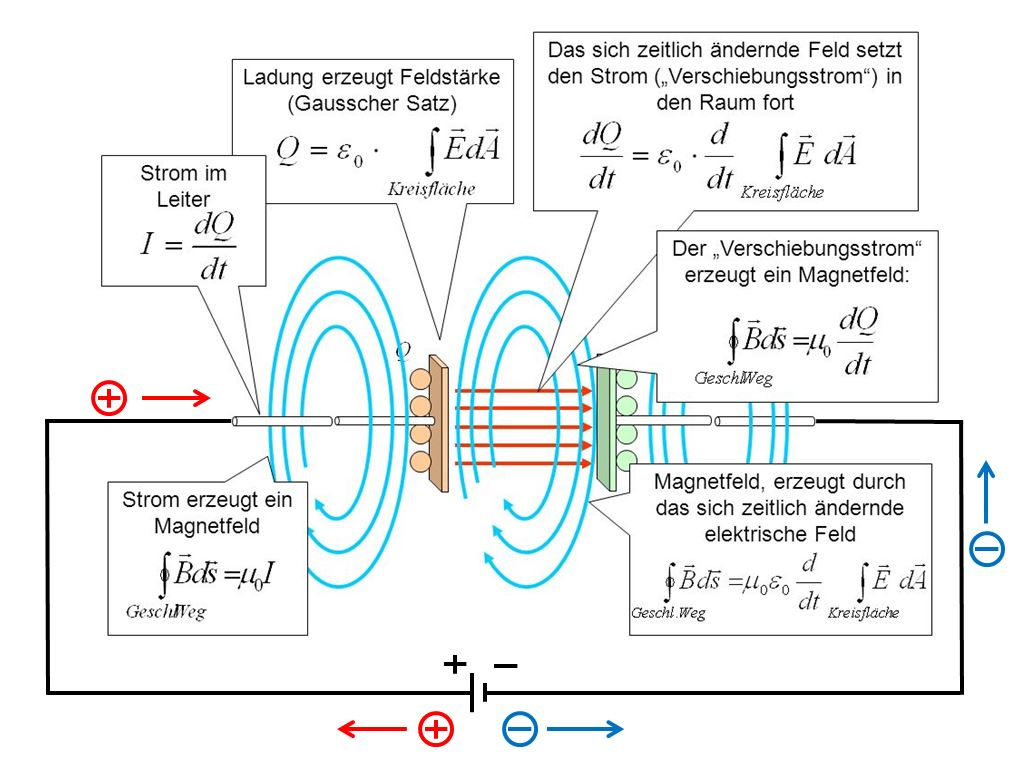
\includegraphics[width=0.8\linewidth]{./pics/el/Iv}
				\caption{Aufladung eines Kondensators als Paradebeispiel für Verschiebungsstrom}
				\label{}
			\end{figure}	
		
		\subsection{Wirbelströme}
			Wie im Induktionsgesetz beschrieben, wird in einem elektrischer Leiter ein Strom induziert wenn sich dieser in einem konstanten Magnetfeld bewegt oder sich in Ruhe in einem sich wechselnden Magnetfeld befindet (= magnetische Flussänderung). Bei einem Draht ist die Stromrichtung eindeutig vorgegeben. Handelt es sich jedoch um einen Leiter mit großer Oberfläche, dann bilden die induzierten Ströme sogenannte Ringströme/Wirbelströme. 
			\begin{figure}[h]
				\centering
				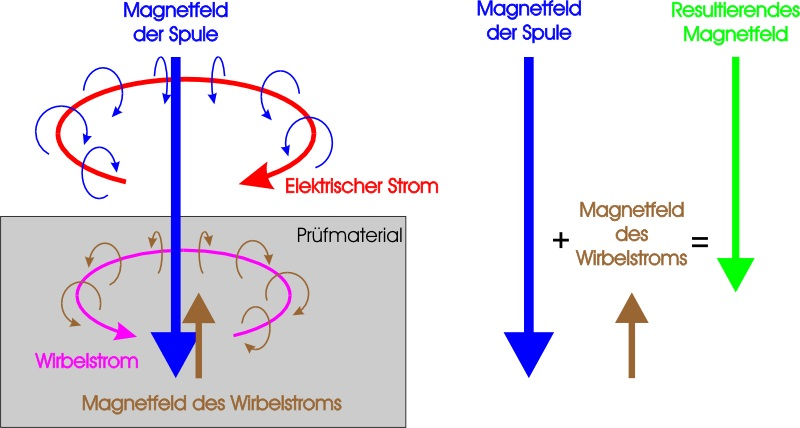
\includegraphics[width=0.7\linewidth]{./pics/el/Wirbel2.jpg}
				\caption{Induktion eines Wirbelstromes}
			\end{figure}
			\leavevmode \\
			Dies ist beispielsweise bei Transformatoren oder Generatoren der Fall. Da Wirbelströme zu Energieverlusten führen, müssen diese durch etwa die Verwendung von Blechpaketen statt einem dicken Eisenkern, reduziert werden. Dabei sind einzelne Bleche elektrisch voneinander isoliert.
		
		\subsubsection*{Wirbelstrombremse}
			Die Wirbelstrombremse ist eine verschleißfreie Bremse. Befindet sich eine Metallplatte in einem inhomogenen Magnetfeld oder wird eine solchige durch ein homogenes Magnetfeld bewegt, werden Wirbelströme induziert. Da die Metallplatte einen ohmschen Widerstand hat, wird die Platte durch die Elektronenbewegung erwärmt. Dies hat zur Folge, dass die Bewegungsenergie der Relativbewegung zwischen Magnetfeld und Metallplatte in Wärmeenergie dissipiert wird. Vorraussetzung für die Induktion von Wirbelströmen, ist das vorhanden sein von freien Ladungsträgern in der Metallplatte (elektrischer Leiter).
			\begin{figure}[h]
				\centering
				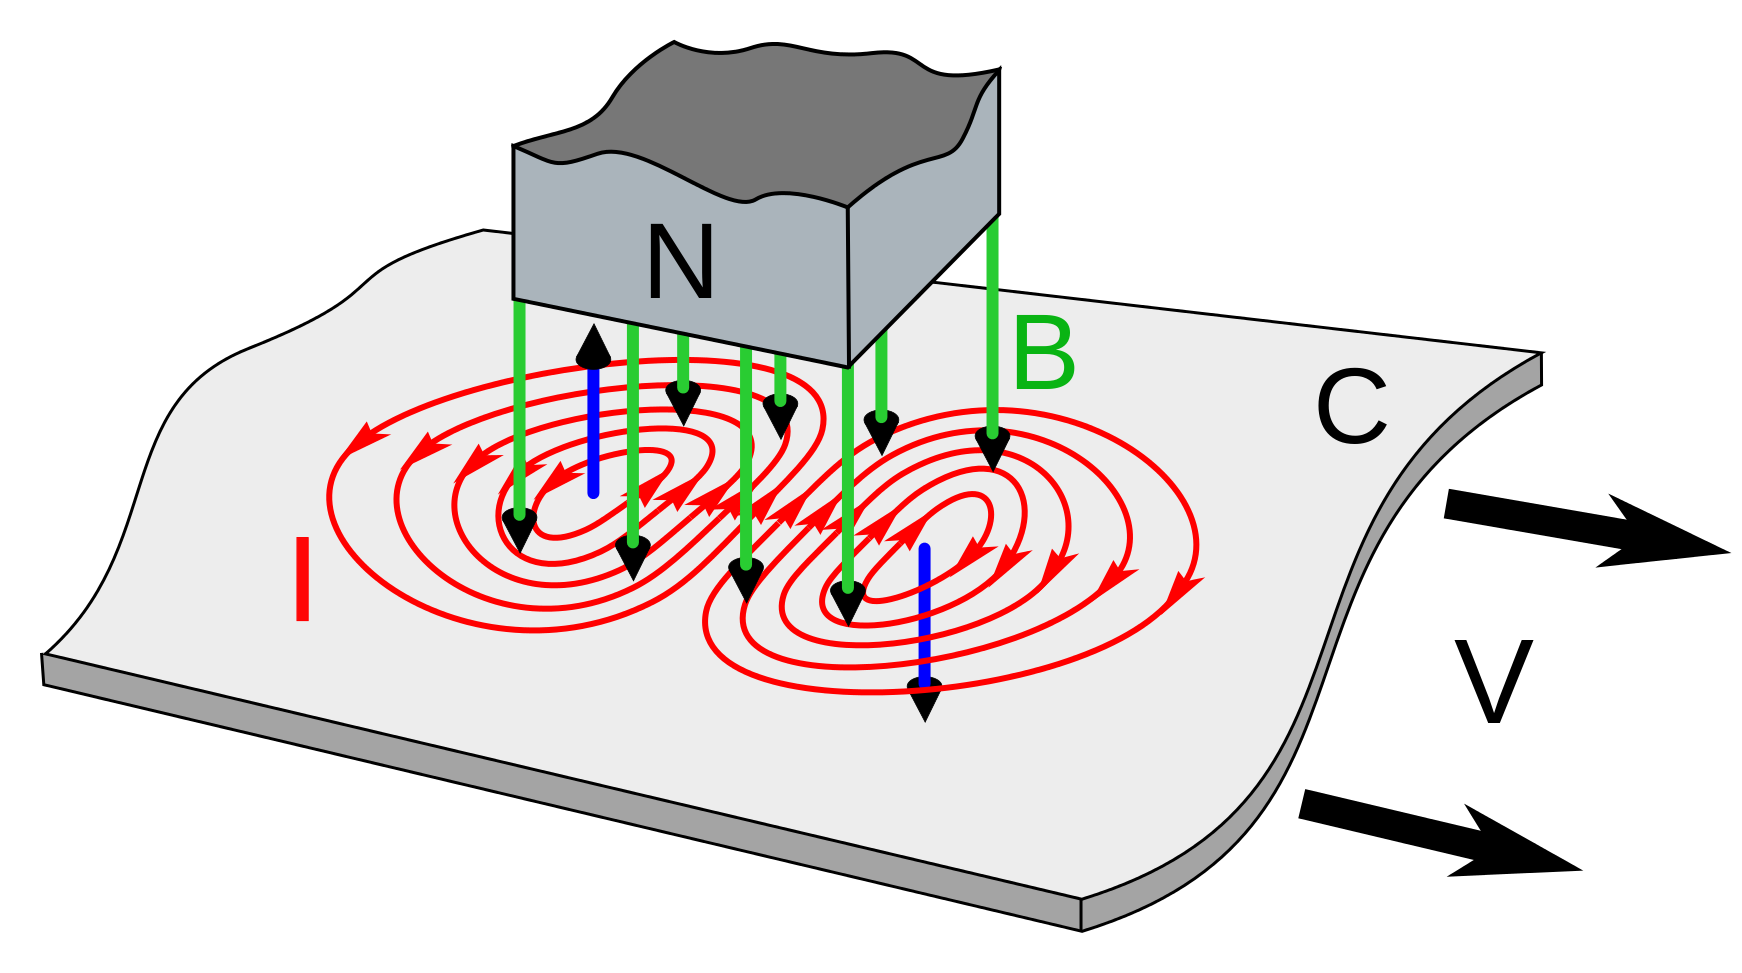
\includegraphics[width=0.49\linewidth]{./pics/el/wirbelbrems1}
				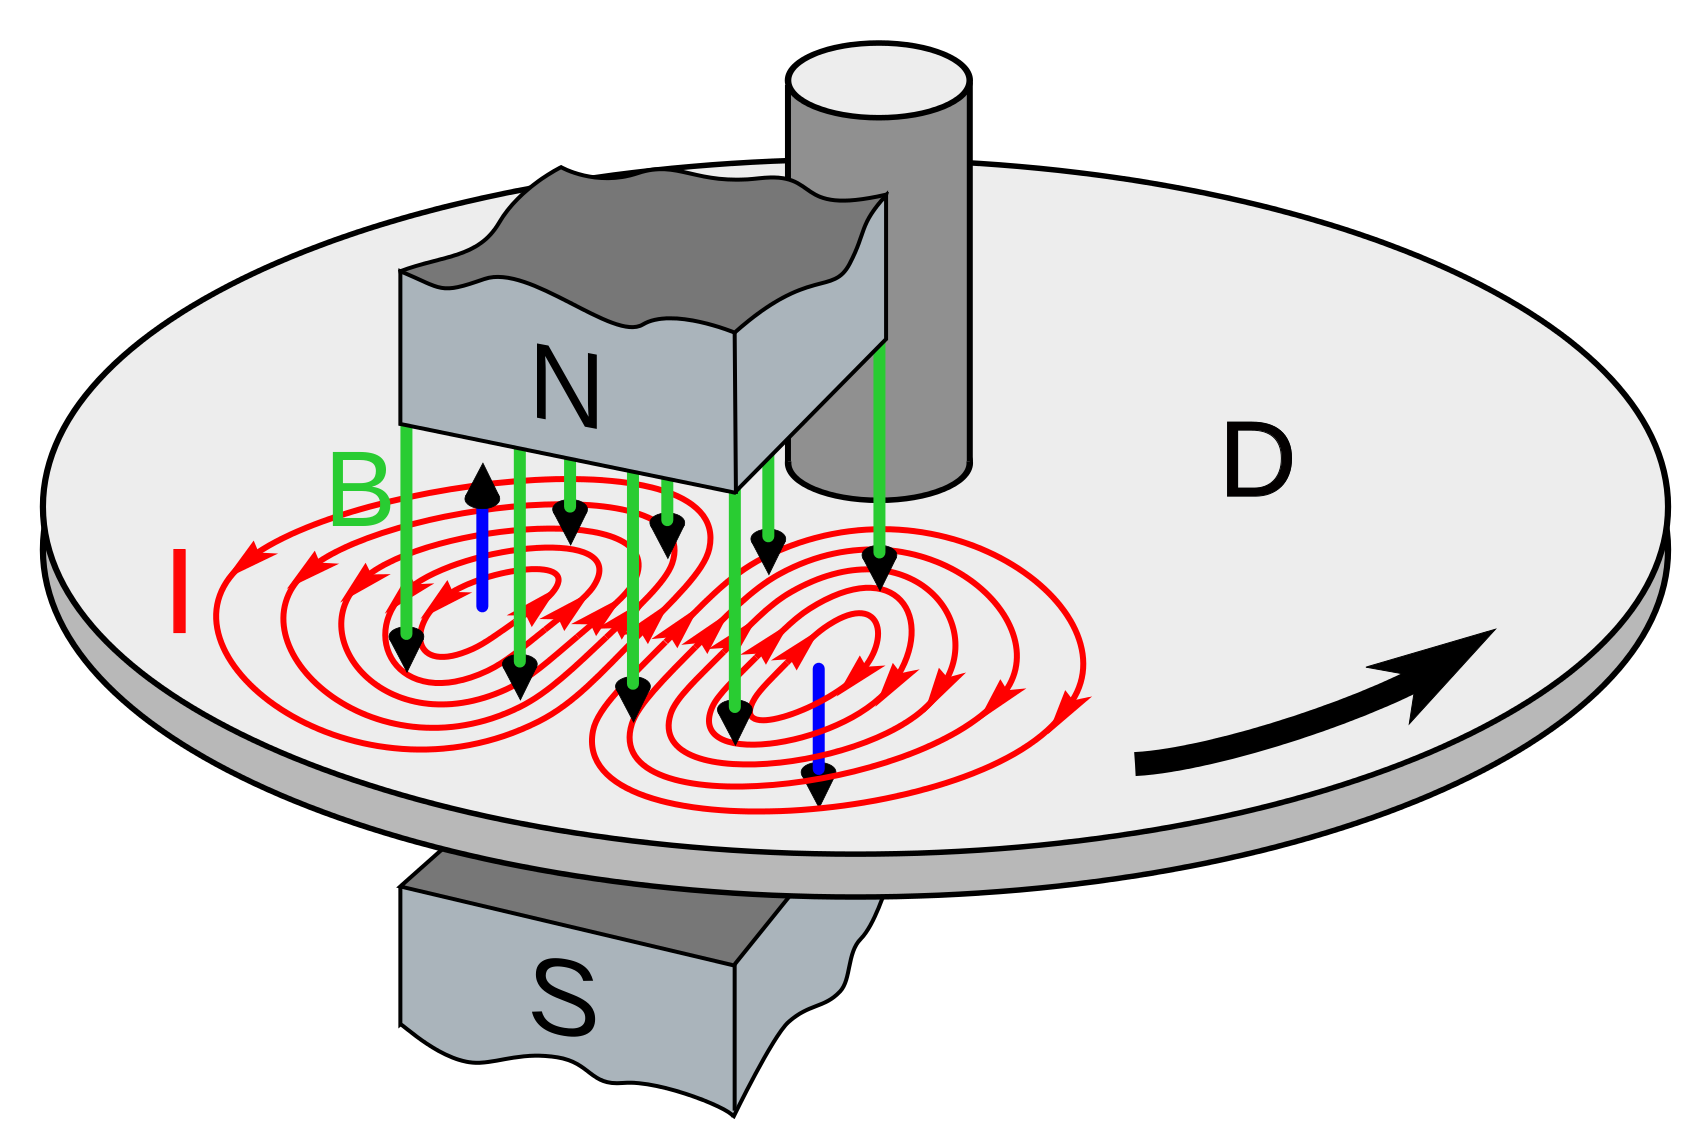
\includegraphics[width=0.49\linewidth]{./pics/el/wirbelbrems2}
				\caption{Beispiele für Wirbelstrombremsen: Zug an Schienen oder LKW an Bremsscheiben}
			\end{figure}
	
		\subsection{Reluktanzkraft/ Maxwellkraft-Prinzip} \label{reluktanzkraft}
			Bei einer stromdurchflossenen Spule, die wie in der Abbildung um einen Eisenkern gewickelt ist, erzeugt die Spule einen magnetischen Fluss im Eisenkern. Es entstehen in beiden Luftspaleten Anziehungskräfte auf den losen Eisenkörper (Anker). Der Effekt der Anziehung beruht darauf, dass die \textit{Reluktanz}, also der magnetishe Widerstand, reduziert und die Induktivität erhöht wird. Das ist der Fall wenn die Feldlinien durch den Anker verlaufen. Wird der Abstand zwischen dem Anker und den Magnetpolen verkürzt, verringert sich der magnetische Widerstand der Feldlinien, denn der Widerstand ist im Eisen wesentlich kleiner als in der Luft.
			\begin{figure}[h]
				\centering
				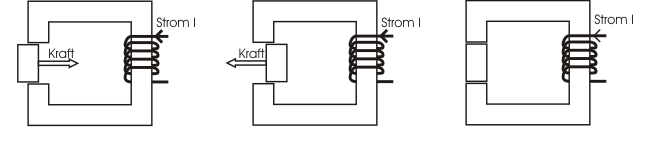
\includegraphics[width=0.7\linewidth]{./pics/el/reluktanz}
			\end{figure}
	
		\subsection{Halbleiter}
			Halbleiter sind Festkörper, deren elektrische Leitfähigkeit zwischen der von elektrischen Leitern und der von Nichtleitern liegt. Da sich die Grenzbereiche der drei Gruppen überschneiden, ist der negative Temperaturkoeffizient des spezifischen Widerstandes ein weiteres wichtiges Merkmal von Halbleitern, das heißt, ihre Leitfähigkeit nimmt mit steigender Temperatur zu, sie sind sogenannte Heißleiter. Ursache hierfür ist die sogenannte Bandlücke zwischen dem Valenz- und dem Leitungsband. Nah am absoluten Temperaturnullpunkt sind diese voll- bzw. unbesetzt und Halbleiter daher Nichtleiter. Es existieren im Gegensatz zu Metallen primär keine freien Ladungsträger, diese müssen erst z. B. durch thermische Anregung entstehen. Die elektrische Leitfähigkeit von Halbleitern steigt aber steil mit der Temperatur an, so dass sie bei Raumtemperatur, je nach materialspezifischem Abstand von Leitungs- und Valenzband, mehr oder weniger leitend sind. Des Weiteren lässt sich durch das Einbringen von Fremdatomen (Dotieren) aus einer anderen chemischen Hauptgruppe die Leitfähigkeit und der Leitungscharakter (Elektronen- und Löcherleitung) in weiten Grenzen gezielt beeinflussen.\\
			Am bekanntesten sind die Elementhalbleiter Silicium und Germanium, die aus einem einzigen Element aufgebaut sind, und Verbindungshalbleitern wie zum Beispiel der III-V-Verbindungshalbleiter Galliumarsenid. Des Weiteren haben in den letzten Jahrzehnten organische Halbleiter an Bedeutung und Bekanntheit gewonnen, sie werden beispielsweise in organischen Leuchtdioden (OLEDs) eingesetzt.
			\begin{itemize}
				\item \textbf{Elementhalbleiter}: Si, Ge, B, Se, Te, C
				\item \textbf{Verbindungshalbleiter}: GaAs, ...
				\item \textbf{Organische Halbleiter}
			\end{itemize}
			\begin{figure}[h]
				\centering
				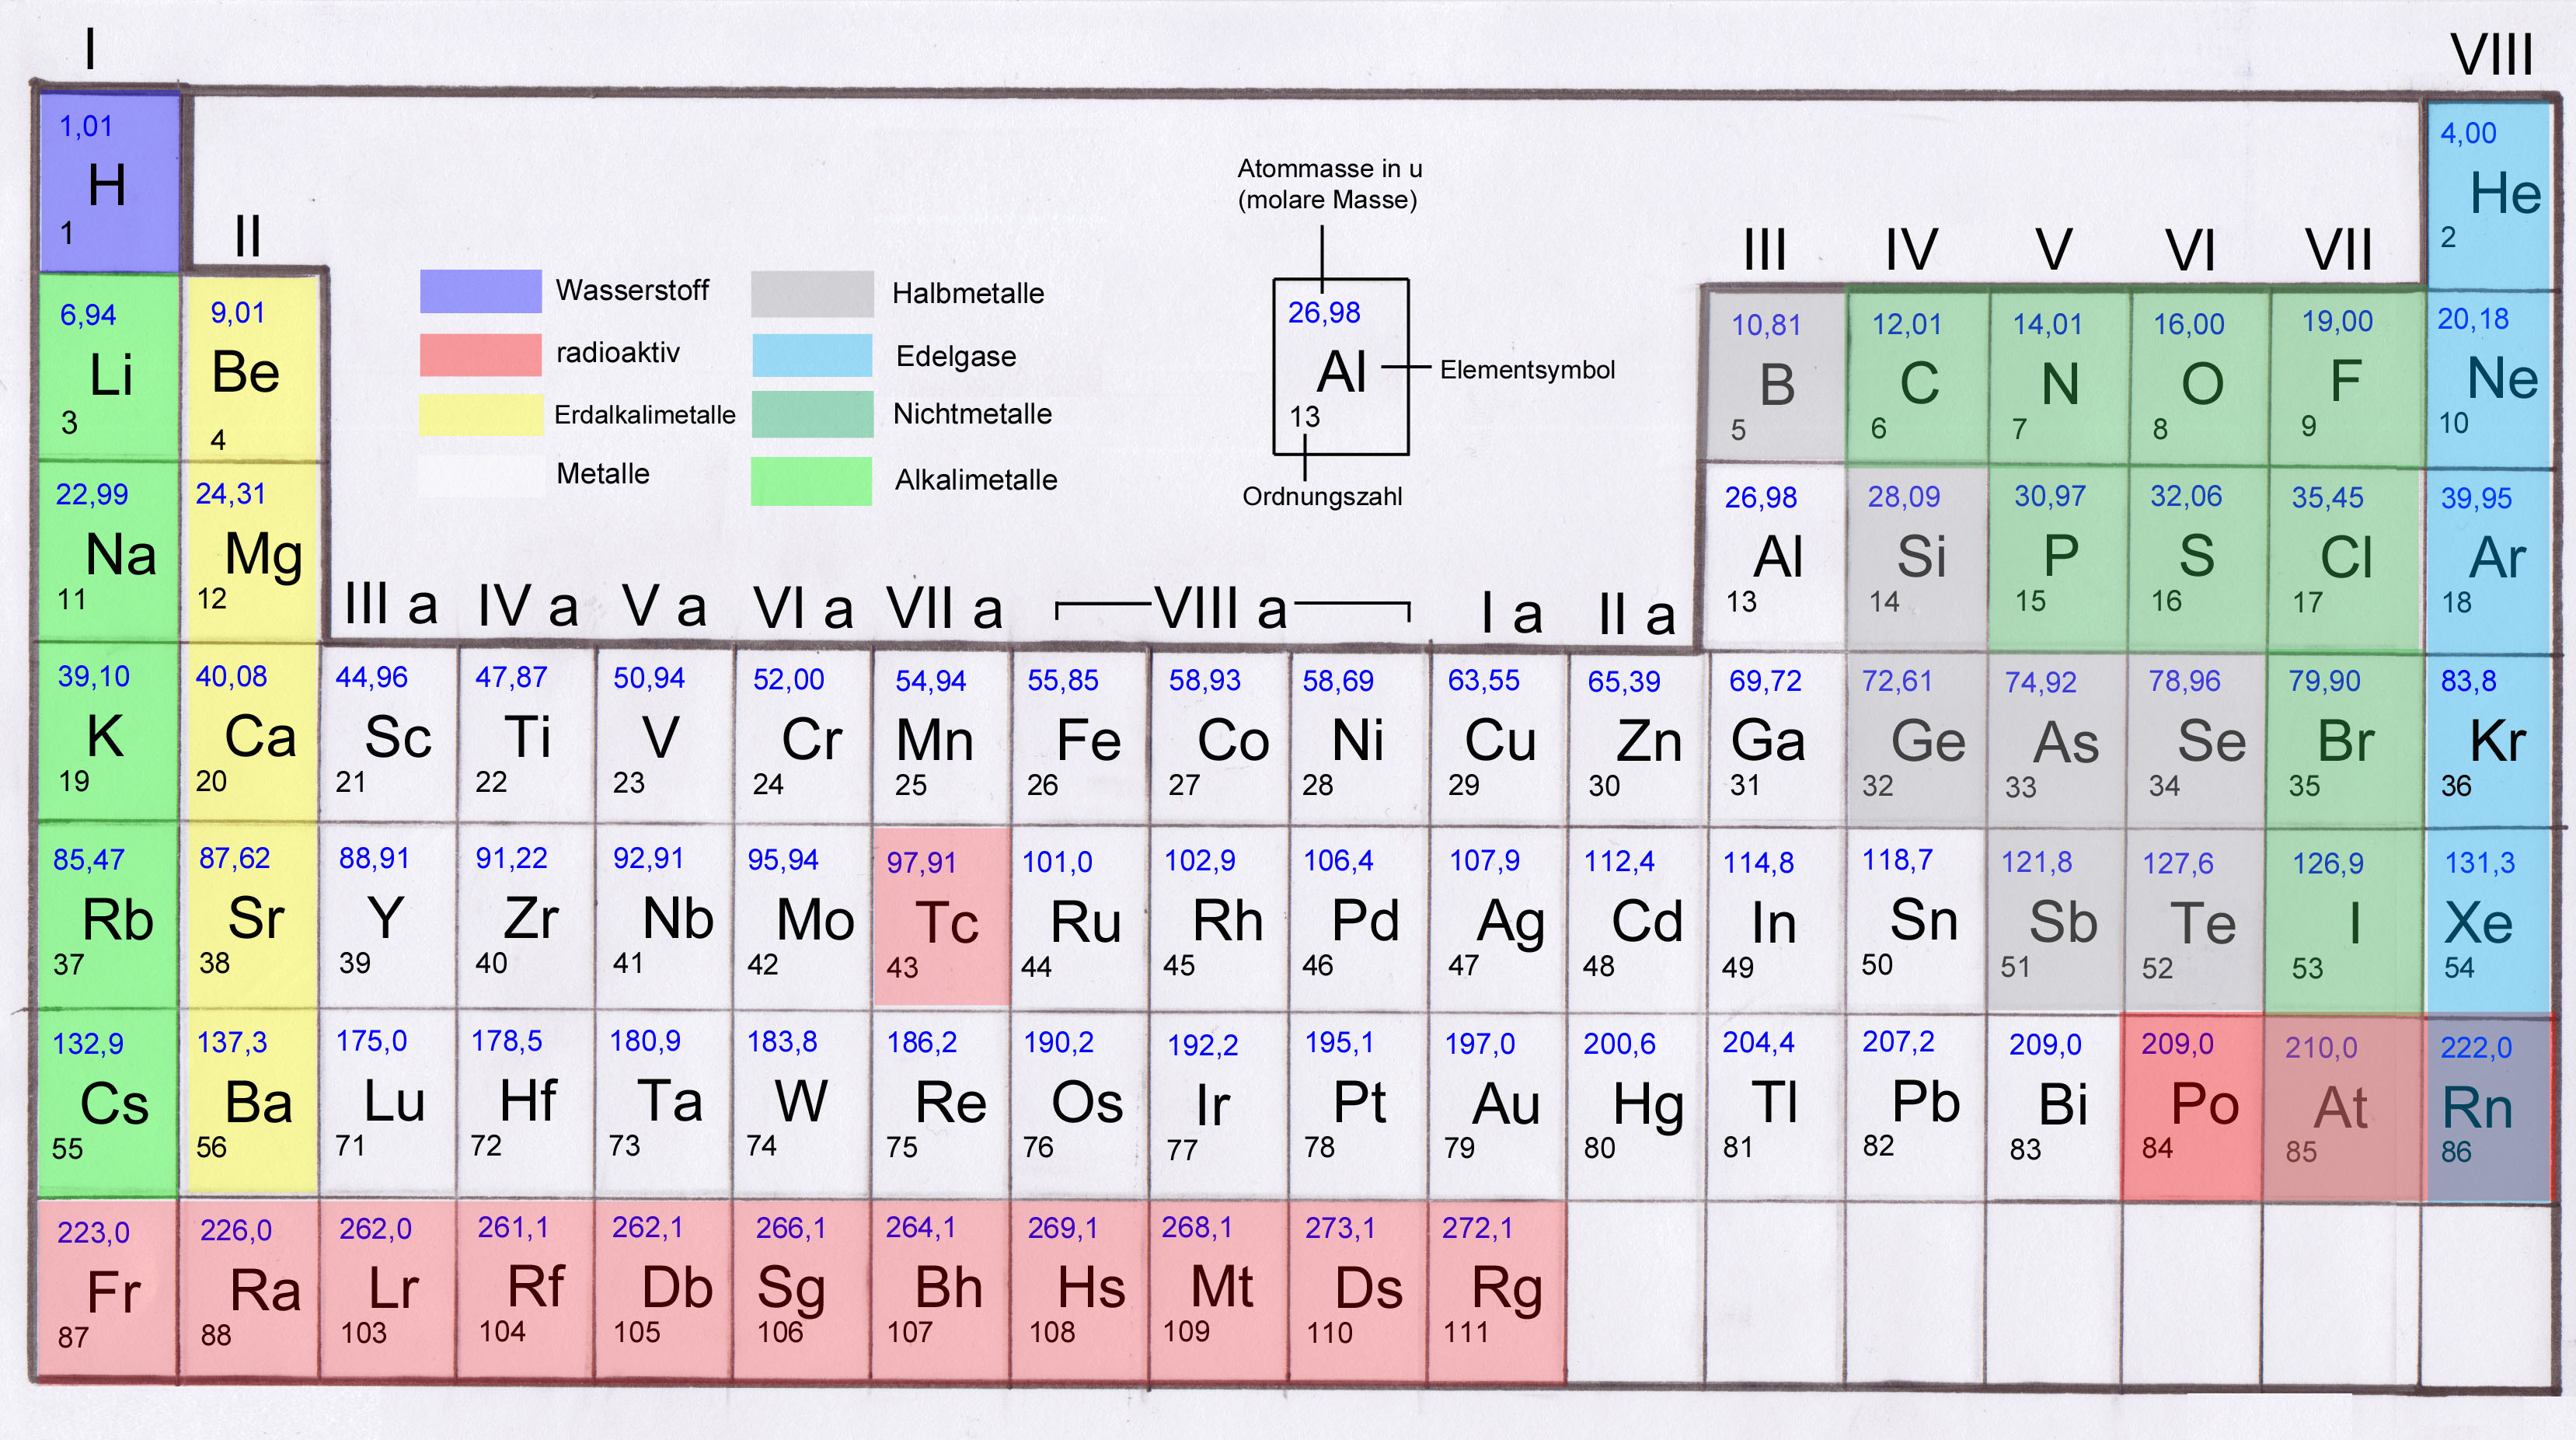
\includegraphics[width=0.73\linewidth]{./pics/el/periodensys}
			\end{figure}

		\subsection{Raumladungszone und p/n-Übergang}
			Für die Herstellung eines Halbleiterbauelements wird der Siliziumkristall verunreinigt. Bei der p-Dotierung werden Fremdatome (Bor) eingefügt die weniger Elektronen als das Silizium besitzen, wodurch sich positive Löcher im Material ausbilden. Bei der n-Dotierung wird Phosphor eingebracht, das mehr Elektronen als das Silizium besitzt und es entsteht ein Material das freie Elektronen besitzt. Dotierte Halbleiter sind in ihrem Grundzustand ungeladen. Es existieren immer gleich viele freie Ladungsträger als ortsfeste Raumladungen der ionisierten Dotierungsatome.
			\begin{figure}[h]
				\centering
				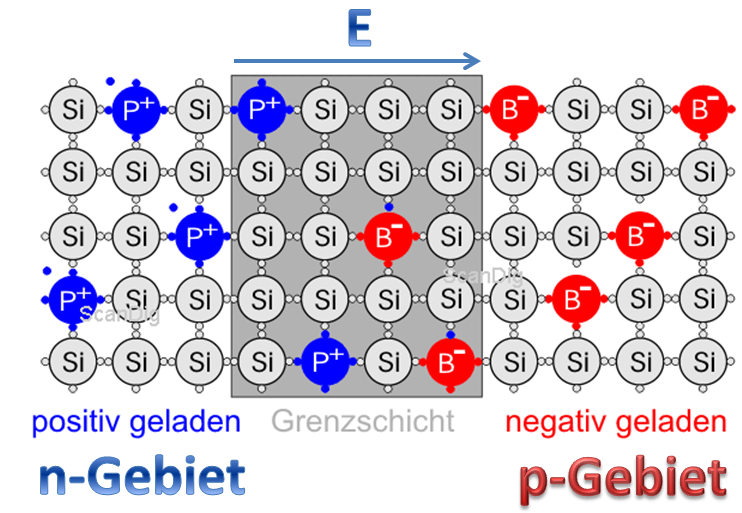
\includegraphics[width=0.4\linewidth]{./pics/el/si}
				\caption{Phosphor mit 5 Protonen im Kern und Bor mit 3 Protonen im Kern, Silizium mit 4 Protonen und Elektronen}
			\end{figure}
			Bringt man diese beiden Materialen aneinander, ergibt sich ein Konzentrationsunterschied von positiven und negativen Ladungsträgern zwischen den beiden Gebieten. Aufgrund von Diffusion streben positive Löcher vom p-dotierten Bereich ins n-Gebiet und negative Elektronen in den p-dotierten Bereich. Positive Löcher rekombinieren im n-Gebiet mit den Elektronen und die Elektronen rekombinieren im p-Gebiet mit den dort vorhandenen Löchern. Es entsteht eine Zone ohne freie Ladungsträger, aber mit positiven Phosphor-Ionen und negativen Bor-Ionen. In weiterer Folge bildet sich ein elektrisches Feld in der Raumladungszone aus. Ist das elektrische Feld groß genug (~0.7V), können die Elektronen des n-Gebiets die Schicht an negativen Bor-Ionen nicht mehr durchdringen und werden von diesen abgestoßen. Das elektrische Feld wirkt der Diffusion entgegen und es hat sich ein Gleichgewicht ausgebildet.
			\subparagraph*{Extern angelegte Spannung} 
				In Durchlassrichtung wirkt das elektrische Feld der externen Spannung, dem elektrischen Feld in der Raumladungszone entgegen. Die positiven Löcher werden vom positiven Pol abgestoßen und die Elektronen vom negativen Pol. Dadurch bewegen sich Elektronen und Löcher zur Mitte Richtung Grenzschicht hin und rekombinieren dort fortlaufend. Ein elektrischer Stromfluss ist möglich. Bei Sperrrichtung liegt genau der umgekehrte Fall vor und die Raumladungszone wird dabei vergrößert.
				\begin{figure}[h]
					\centering
					\subfigure[Durchlassrichtung]
					{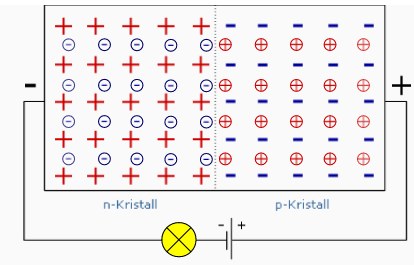
\includegraphics[width=0.35\textwidth]{./pics/el/durchlass}} \hspace{0.4cm}
					\subfigure[Sperrrichtung] 
					{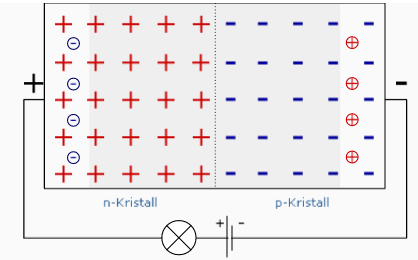
\includegraphics[width=0.35\textwidth]{./pics/el/sperr}}
				\end{figure}

		
	
	\newpage
	\section{Elektrische Bauelemente}
		\subsection{Bipolar-Transistor}
			\subsubsection*{Funktionsweise}
				Im Folgenden wird die physikalische Stromrichtung (Elektronenstrom) für die Erläuterung verwendet. Durch das Anlegen einer Spannung $ U_{BE} $ von etwa 0,7 V, ist die untere Diode (Prinzip) in Durchlassrichtung geschaltet. Die Elektronen gelangen in die p-Schicht und werden von dem Plus-Pol der Spannung $ U_{BE} $ angezogen.
				Da die p-Schicht sehr klein ist, wird nur ein geringer Teil der Elektronen angezogen.
				Der größte Teil der Elektronen bewegt sich weiter in die obere Grenzschicht. Dadurch wird diese leitend und der Plus-Pol der Spannung $ U_{CE} $ zieht die Elektronen an. Es fließt ein Kollektorstrom $ I_{C} $.
				Bei üblichen Transistoren gelangen etwa 99\% der Elektronen von Emitter zum Kollektor durch. In der Basisschicht rekombinieren etwa 1\% der Elektronen.
				\begin{figure}[h]
					\centering
					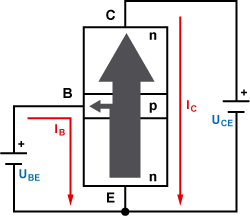
\includegraphics[width=0.4\linewidth]{./pics/el/npn.png}
				\end{figure}
			
	\section{\textcolor{red}{Elektronische Grundschaltungen}}
		\subsection{\textcolor{red}{Wechselrichter}}
			\begin{figure}[h]
				\centering
				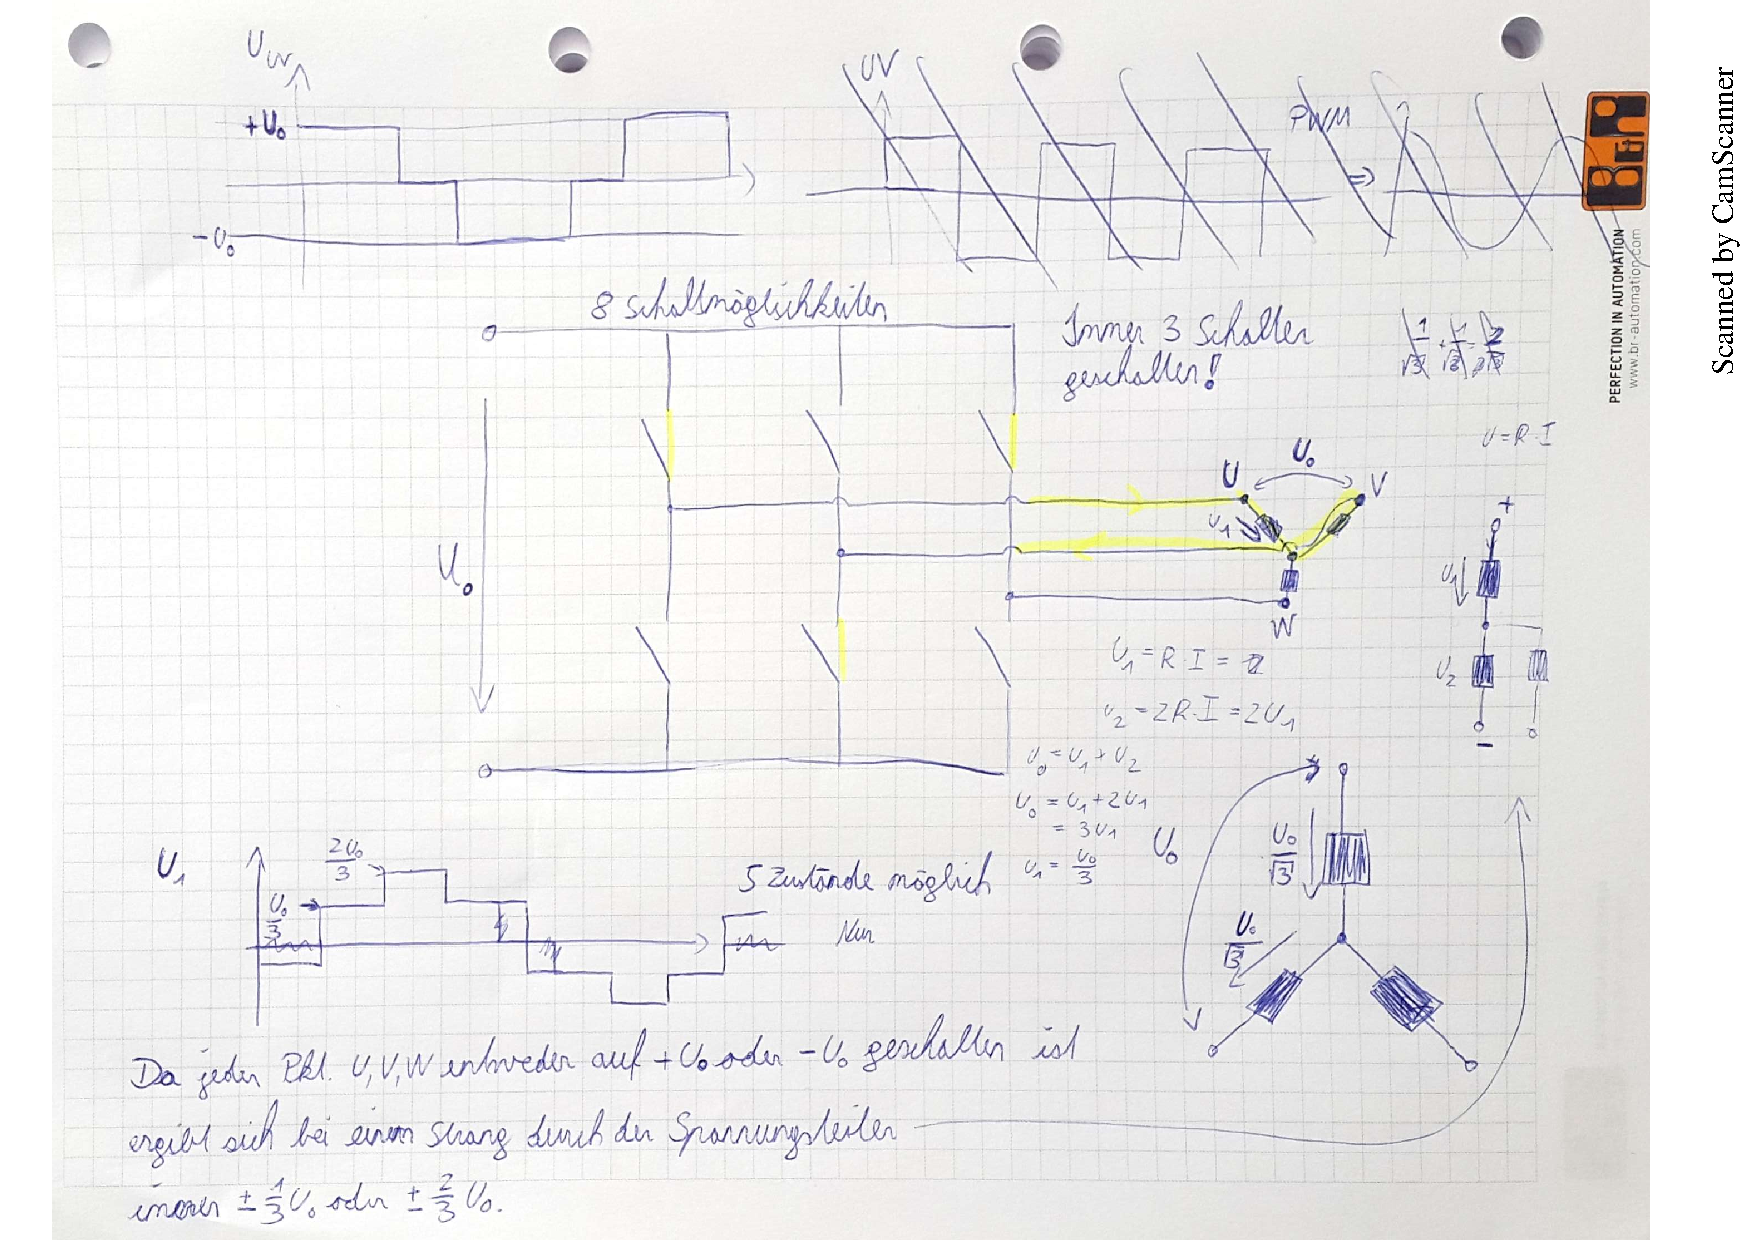
\includegraphics[width=1\linewidth]{./pics/el/wechsel.pdf}
				\caption{}
				\label{}
			\end{figure}
			\begin{figure}[h]
				\centering
				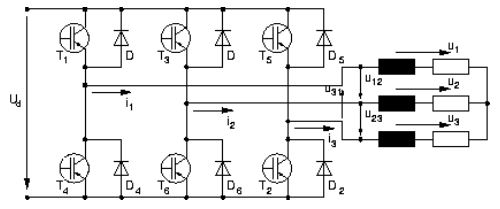
\includegraphics[width=0.5\linewidth]{./pics/el/wechsel1}
				\caption{}
				\label{}
			\end{figure}
			\begin{figure}[h]
				\centering
				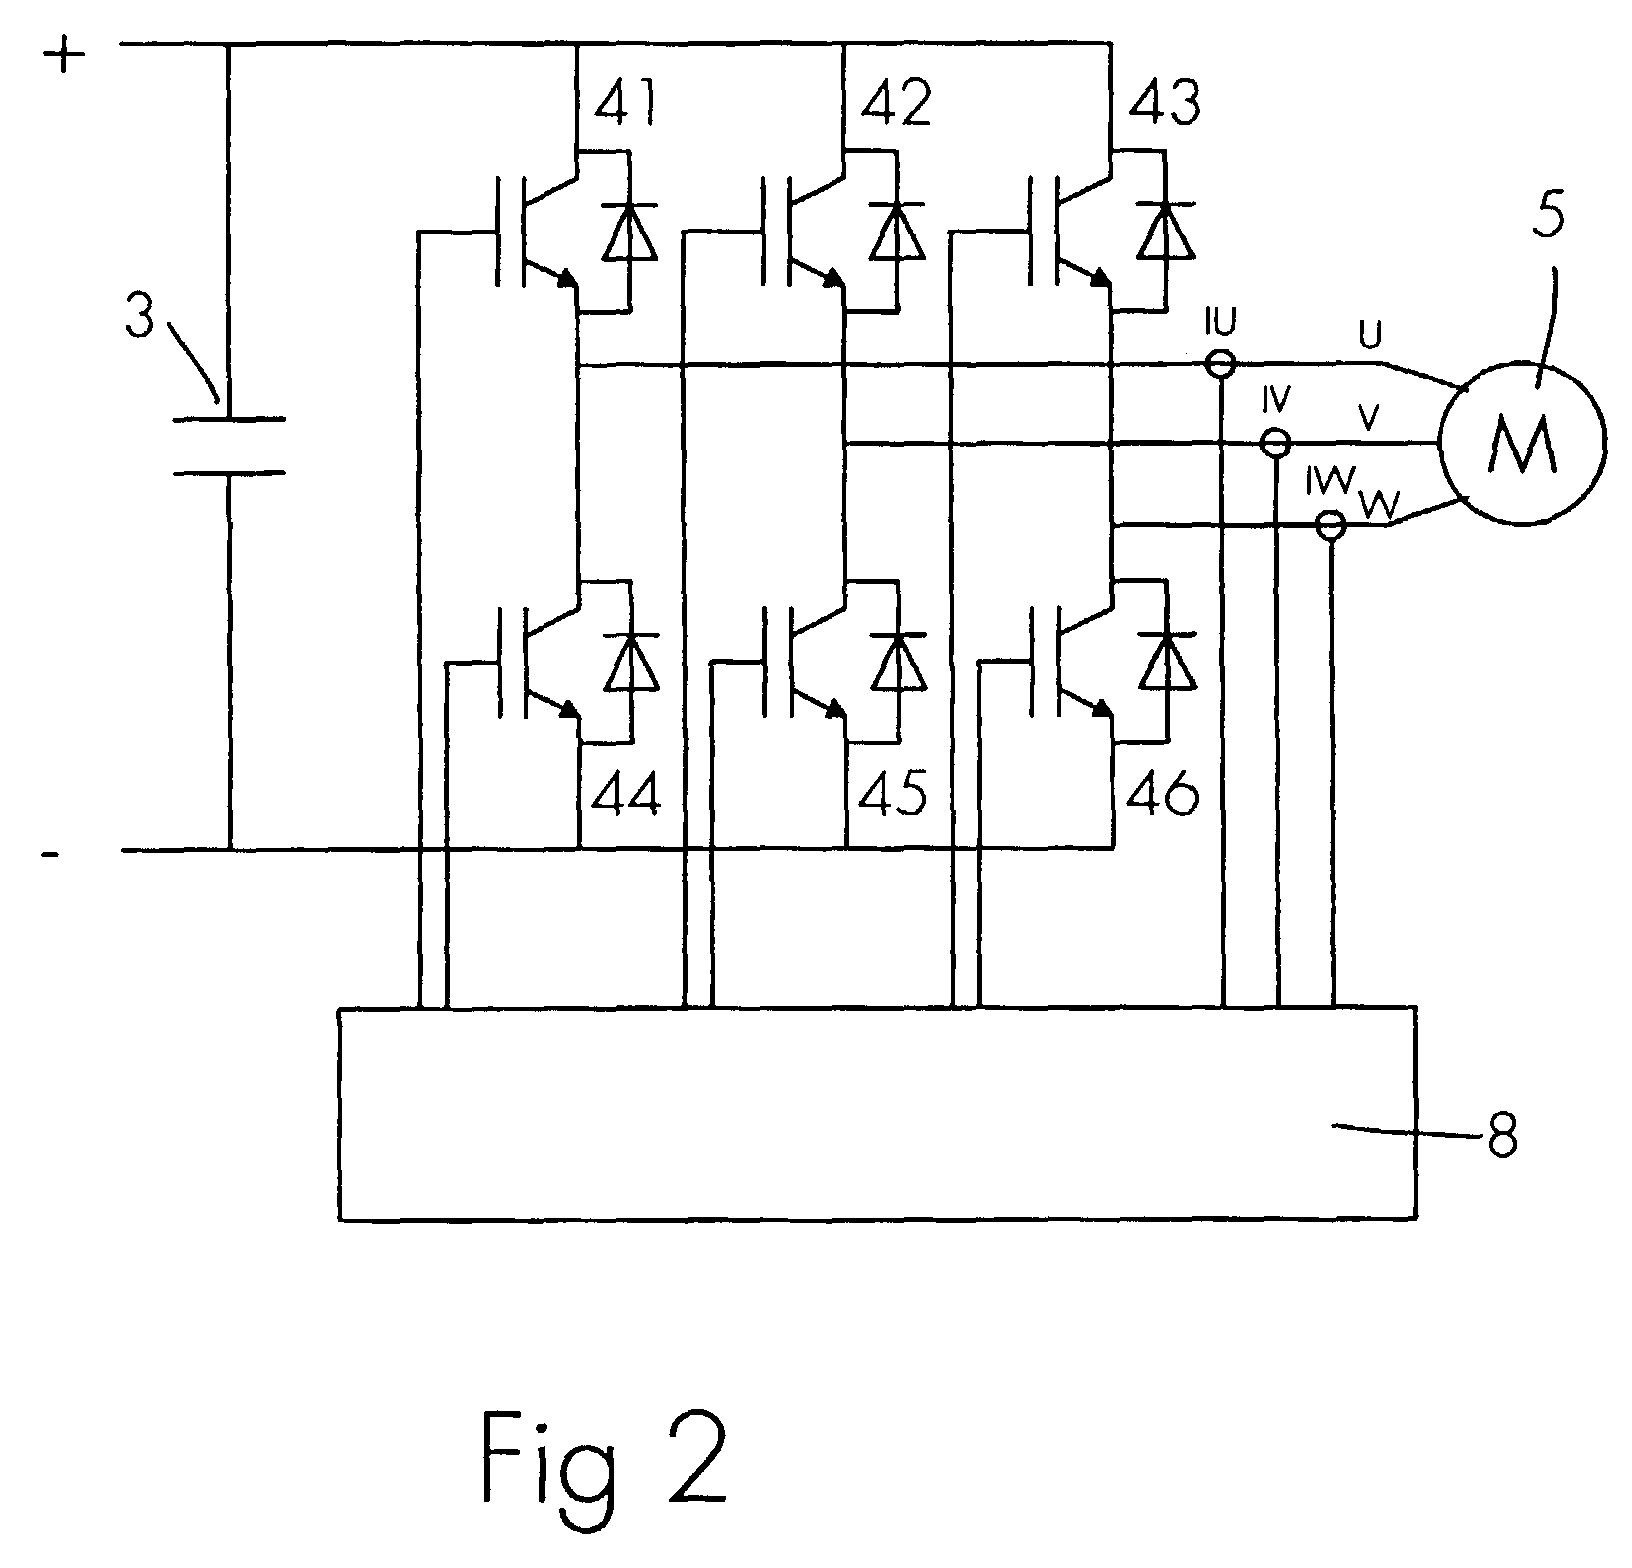
\includegraphics[width=0.5\linewidth]{./pics/el/wechsel2}
				\caption{}
				\label{}
			\end{figure}
			\leavevmode \\
	\section{\textcolor{red}{Filter}}
		\subsection{Filtertypen}
		\begin{itemize}
			\item Tiefpassfilter
			\item Hochpassfilter
			\item Bandpassfilter
			\item Bandsperre, Kerbfilter
			\item Allpassfilter – lässt alle Frequenzen mit gleicher Verstärkung durch, kann aber eine Phasenverschiebung verursachen.
		\end{itemize}
		Die Filterordnung beschreibt die Dämpfung von Frequenzen unterhalb od. oberhalb der Grenzfrequenz. Z.b. bei einem Filter n. Ordnung würde die TF mit $ n\cdot6dB/Oktave $ fallen.\\\\
		Weitere Einteilungen: Aktiv, Passiv, Linear, Nicht-Linear, Ordnung
		\subsection{\textcolor{red}{Analoges aktives Filter}}
		\subsection{\textcolor{red}{Analoges passives Filter}}
			\subsubsection{\textcolor{red}{Topologien}}
			https://de.wikipedia.org/wiki/Analogfilter\\
			http://elektroniktutor.de/analogtechnik/filter.html
			\subsubsection{\textcolor{red}{Tiefpassfilter}}
				Praktische Anwendung, wie wird ein Tiefpassfilter dimensioniert --> gewünschte Grenzfrequenz einstellen
			\subsubsection{\textcolor{red}{Hochpassfilter}}
			\subsubsection{Notchfilter}
				Ein Kerbfilter ist ein elektronisches Filter, mit dem Frequenzen innerhalb eines engen Frequenzbereiches ausgefiltert werden können. Anschaulich wird eine Kerbe in das Frequenzdiagramm eingefügt.
				Kerbfilter stellen einen besonders schmalbandigen Typ von Bandsperrfilter dar, welche in der Übertragungsfunktion nur eine Nullstelle aufweisen und damit nicht ein breites Frequenzband, sondern idealerweise genau eine Frequenz möglichst stark dämpfen.
				
		\subsection{\textcolor{red}{Digitales Filter}}
			\subsubsection{\textcolor{red}{FIR - Finite Impulse Response}}
			\subsubsection{\textcolor{red}{IIR - Infinite Impulse Response}	}		
		\subsection{Kalmanfilter}
			Ein Kalman-Filter schätzt den Wert einer ungenauen oder unsicheren Messung anhand der vorhergegangen Messwerte ab. Das Prinzip beruht auf Wahrscheinlichkeitsfunktionen. Systemzustände müssen dafür bekannt sein und fließen in die Berechnung mit ein. Anders formuliert wird eine Vorhersage des nächsten Wertes anhand des momentanen Wertes und der bekannten System-Eingangsvariablen geschätzt. Zusätzlich vergrößern die nicht abschätzbaren Parameter den Wahrscheinlichkeitsbereich, wo der nächste Wert landen könnte. Hinzu kommt nun noch eine Wahrscheinlichkeit für den Messwert des Sensors. Aufgrund von Rauschen erhalten wir einen anderen Wert als real vorhanden ist. Diese Abweichung wird wiederum als Wahrscheinlichkeit beschrieben. Nun kann man die beiden Wahrscheinlichkeiten (die des nächsten Wertes und der Korrektheit des Messwertes) multiplizieren und erhält einen neuen verbesserten Schätzwert.\\
			Dieser verbesserte Schätzwert kann nun wieder durch den ganzen Ablauf verwendet werden und wir erhalten einen neuen Schätzwert. Dieser Vorgang kann beliebig oft vorgenommen werden.
			Die Filter sind sehr schnell – Echtzeitfähig – und liefern in der Praxis sehr gute Ergebnisse. Zeigt sehr gute Filtereigenschaften für Sensorrauschen (Unsicherheit der Messung ausgleichen).\\
			http://www.bzarg.com/p/how-a-kalman-filter-works-in-pictures/
			
	\section{\textcolor{red}{Sensoren}}
		\subsection{\textcolor{red}{Übersicht von Sensoren nach deren Messgrößen}}
		Abstands- bzw. Wegsensoren
		Geschwindigkeits und Drehzahlsensoren
		Beschleunigungssensoren
		\subsection{Encoder}
			\subsubsection{TTL-Encoder}
				2 Signale A,B mit insgesamt 4 verschiedenen Zuständen --> Drehencoder mit 1000 ppr = 4000 Zustände pro Umdrehung.
			\subsubsection{SinCos-Encoder}
		\subsection{\textcolor{red}{Piezoelektrische Sensoren}}
		\subsection{\textcolor{red}{Induktive Sensoren}}
		\subsection{\textcolor{red}{Kapazitive Sensoren}}
		\subsection{\textcolor{red}{Mechanische Sensoren}}
		\subsection{\textcolor{red}{Thermoelektrische Sensoren}}
		\subsection{\textcolor{red}{Resistive Sensoren}}
		\subsection{\textcolor{red}{Magnetische Sensoren}}
		\subsection{\textcolor{red}{Optische Sensoren}}
			\subsubsection{Interferometer}
				Das Messprinzip basiert auf der Überlagerung von zwei Wellen die unterschiedliche Wege zurücklegen. Grundsätzlich lässt sich mit jeder Art von Welle, seien es elektromagnetische Wellen, Schall- oder Materiewellen, eine Interferenz erzeugen.\\ Laserlicht eignet sich ausgezeichnet für kürzere (Meterbereich) und äußerst präzise (Pikometerbereich) Wegmessungen. Voraussetzung für eine erfolgreiche Interferenz ist, dass Wellen kohärent überlagert werden. Deshalb wird Laserlicht verwendet, da ausgesendete Lichtwellen nahezu phasengleich zueinander sind und eine sehr große Kohärenzlänge (max. Weglänge zweier Lichtstrahlen, bei der diese noch ein stabiles Interferenzmuster ergeben) - d.h. auch über große Distanzen phasengleich bleiben - besitzen. \\
				Die unterschiedlichen Typen von Interferometern haben meist das selbe Funktionsprinzip. Durch Überlagerung zweier Wellen, die in getrennten optischen Bahnen geführt und von Spiegeln bzw. einem Objekt reflektiert werden, bilden ein Interferenzmuster (Interferenzstreifen oder -ringe). Dieses ist abhängig von der Distanz des Objektes. Somit können Distanzänderungen detektiert werden.\\
				So werden beim \textbf{Michelson-Interferometer} durch einen Photosensor abwechselnd Minima und Maxima des Interferenzbildes registriert und mitgezählt. Wird die Anzahl der gemessenen Maxima mit der Wellenlänge des Laserlichts multipliziert, erhält man die Wegdifferenz. Da das Medium durch das die elektromagnetische Welle wandert, deren Wellenlänge beeinflusst, ist ein wichtiger Faktor, die Eigenschaften dieses Mediums zu berücksichtigen (Luftdruck, Luftfeuchtigkeit, Temperatur).\\
				Bei Vielstrahlinterferometern wie dem \textbf{Fabry-Per\'{o}t-Interferometer} wird die Längenänderung gemessen indem die Länge des optischen Resonators verändert wird. D.h. ein optischer Ausgang/Messkopf des Interferometers und das Objekt bilden gemeinsam einen optischen Resonator. Martin Zech von Attocube hat ein solches Interferometer entwickelt, das Genauigkeiten im sub-Nanometerbereich bei Raumtemperatur erreicht. Wird der Sensor mit flüssigem Helium auf 4 K gekühlt kann durch Rauschunterdrückung eine Genauigkeit von 1 pm erreicht werden.\\
		
				Vorteil:
				\begin{itemize}
					\item Höhere Empfindlichkeit 
					\item Längenmessungen bis 10$ ^{-12} $ m Genauigkeit können gemessen werden
				\end{itemize}
		
		
		

	\section{Elektrische Maschinen}
		\leavevmode
		\begin{figure}[h]
			\centering
			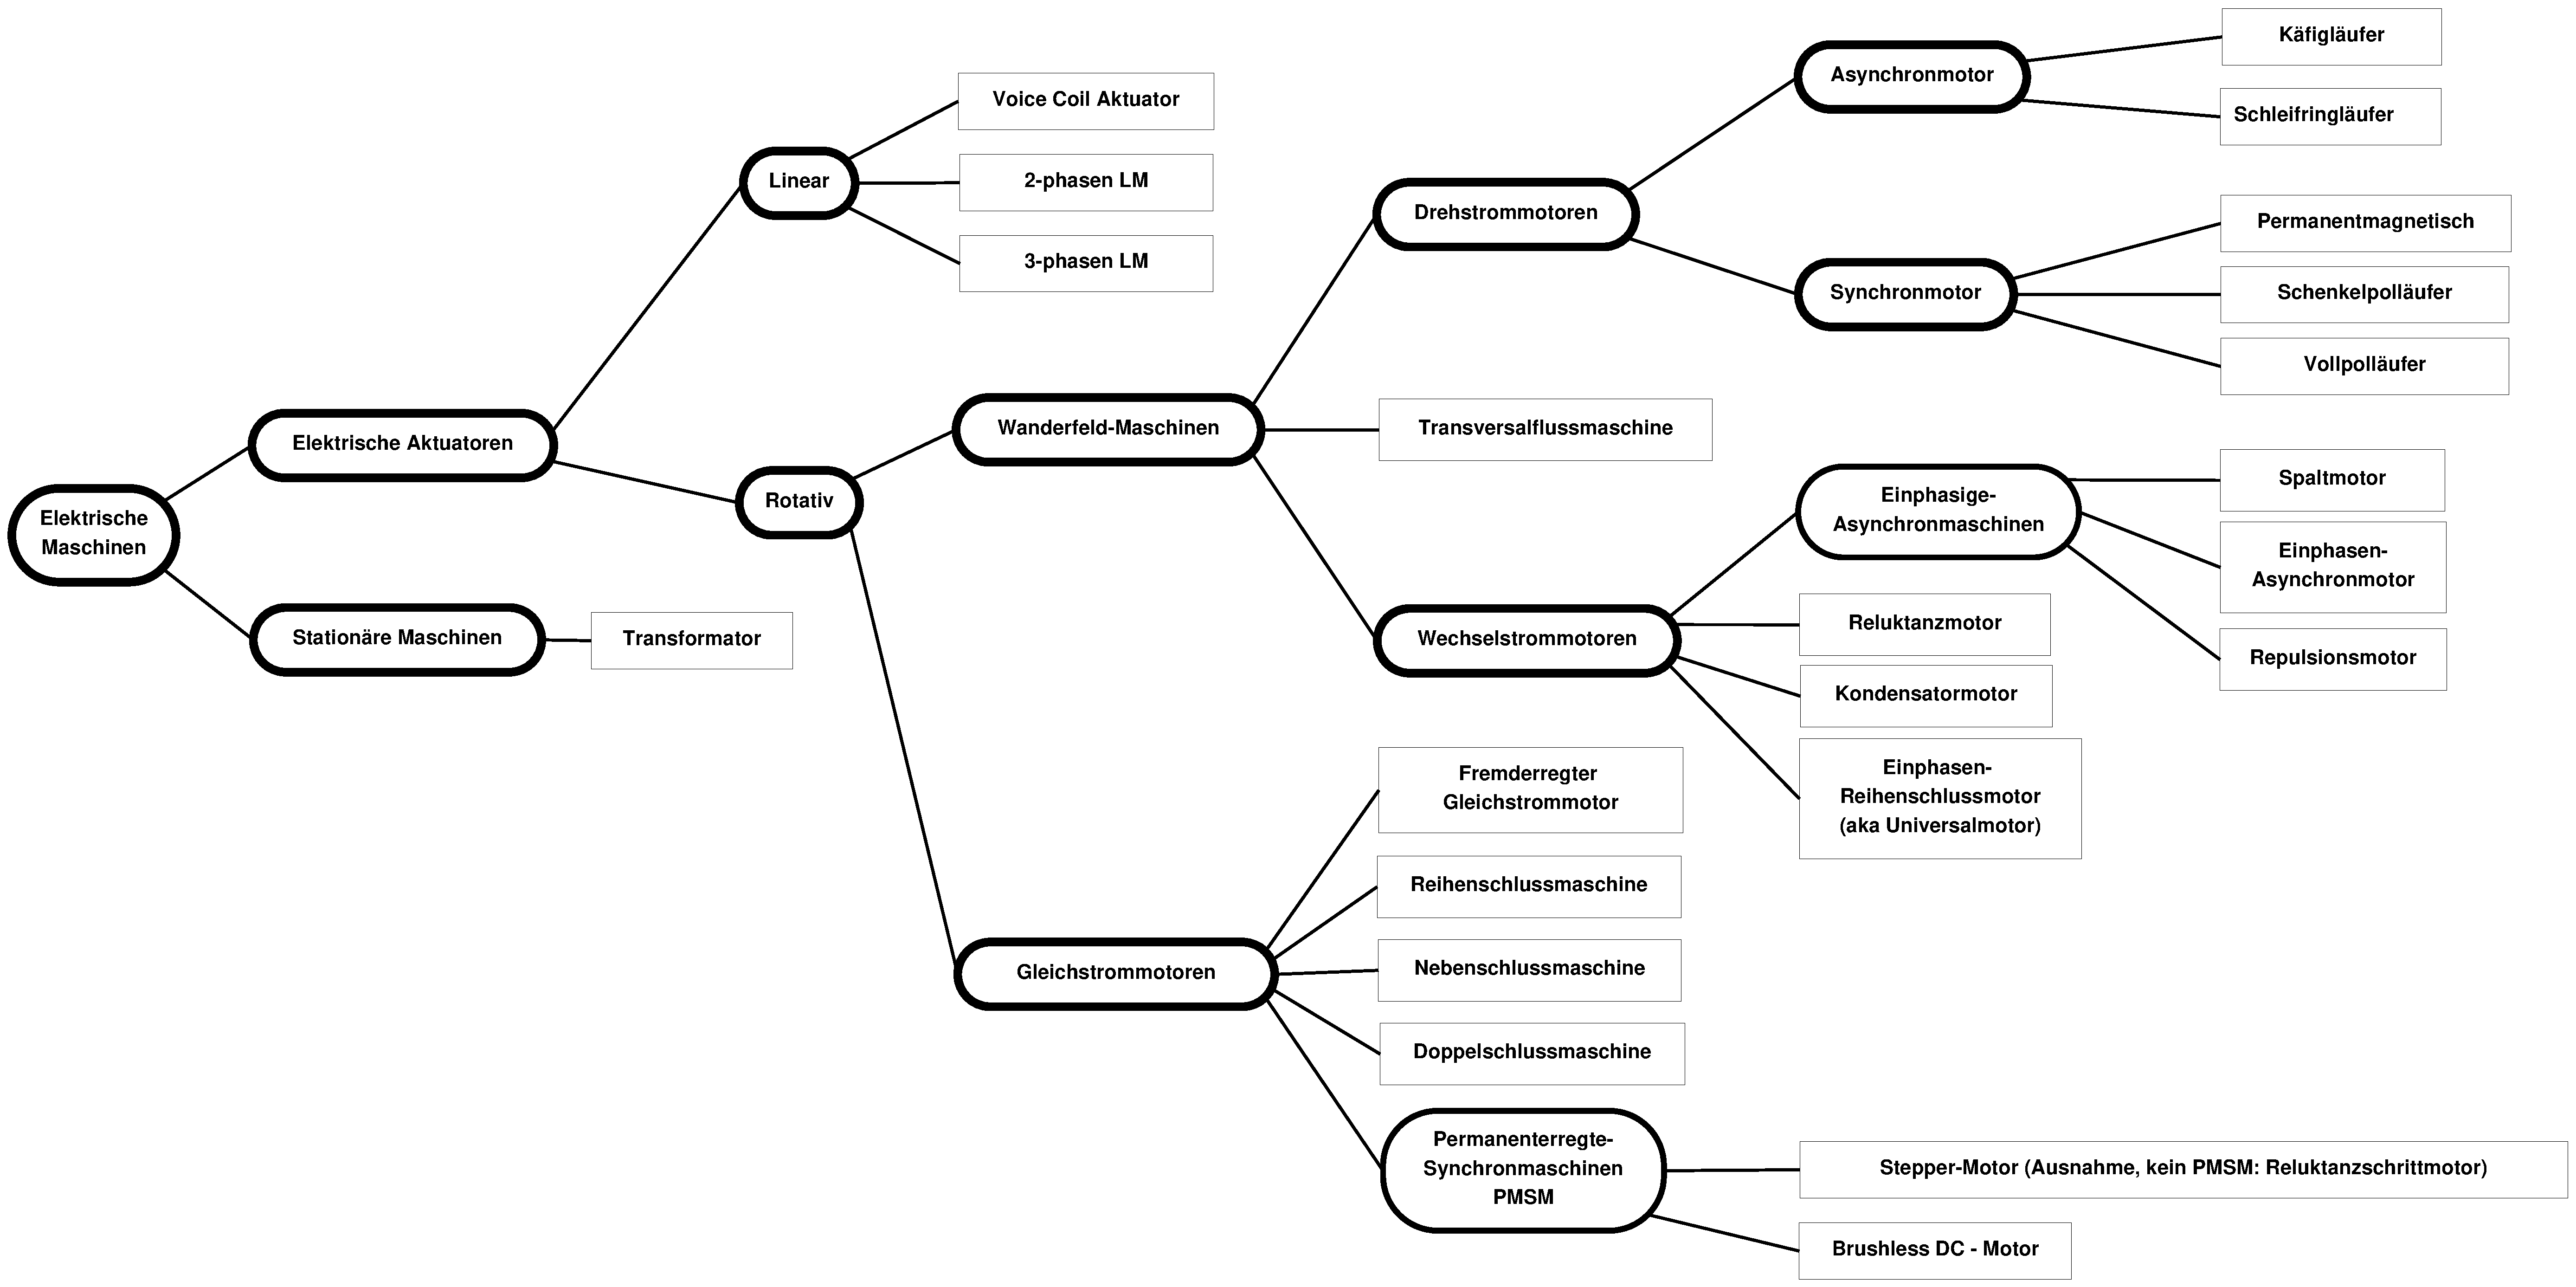
\includegraphics[width=1\linewidth]{./pics/el/elMasch}
		\end{figure}
		\subsection{Stationäre Maschinen}
			\subsubsection{Transformator}
				Ein Transformator besteht meist aus zwei oder mehr Spulen (Wicklungen), die in der Regel aus Kupferdraht gewickelt sind und sich auf einem gemeinsamen Ferrit- bzw. Eisenkern befinden. Ein Transformator wandelt eine Eingangswechselspannung, die an einer der Spulen angelegt ist, in eine Ausgangswechselspannung um, die an der anderen Spule abgegriffen werden kann. Dabei entspricht das Verhältnis von Eingangs- und Ausgangsspannung dem Verhältnis der Windungszahlen der beiden Spulen. So wird zum Beispiel bei einem Windungsverhältnis von 20 zu 1 eine Eingangsspannung von 240 Volt in eine Ausgangsspannung von 12 Volt transformiert. Je nach Auslegung des Transformators kann die Ausgangsspannung somit kleiner, größer oder gleich der Eingangsspannung sein.
				\paragraph*{Wirkprinzip}
					Eine Wechselspannung auf der Primärseite des Transformators bewirkt entsprechend dem Induktionsgesetz einen wechselnden magnetischen Fluss im Kern. Der wechselnde magnetische Fluss wiederum induziert auf der Sekundärseite des Transformators eine Spannung (Spannungstransformation)
					\begin{figure}[h]
					\centering
					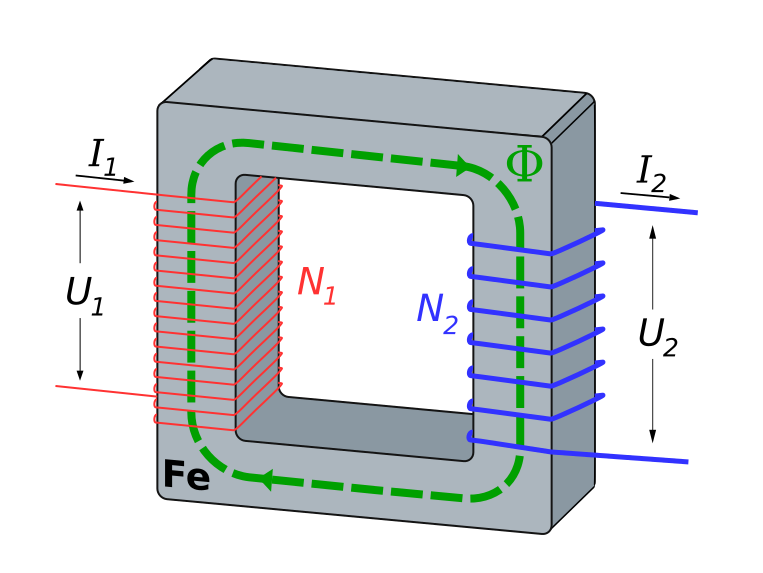
\includegraphics[width=0.4\linewidth]{./pics/el/trafo}
				\end{figure}\\
					Spannungstransformation beim ideal Transformator:\\
					\[\dfrac{U_{2}}{U_{1}}=\dfrac{N_{2}}{N_{1}} \qquad \text{bzw.} \qquad U_{2}=\dfrac{N_{2}}{N_{1}}U_{1}\]
					Wird an die sekundäre Wicklung ein \textbf{Verbraucher angeschlossen}, so entnimmt dieser der Sekundärspule elektrische Energie. Dabei kommt ein Strom auf der Sekundärseite zustande und der Primärstrom vergrößert sich. Im Gegensatz zu den Spannungen an den Wicklungen sind die Ströme in den Wicklungen jedoch entgegengesetzt gerichtet: Wenn der Primärstrom bezogen auf den Kern rechtsherum durch die Spule fließt, fließt der Sekundärstrom linksherum und umgekehrt (Lenzsche Regel).
					\[\dfrac{I_{2}}{I_{1}}=\frac{N_{1}}{N_{2}}\qquad \text{bzw.} \qquad I_{2}=\frac{N_{1}}{N_{2}}I_{1}\]
				\paragraph*{Realer Transformator}
					Ein realer Transformator hat demgegenüber Übertragungsverluste durch den ohmschen Widerstand der Wicklung, durch Wirbelstrombildung im Kern, Ummagnetisierungsverluste und durch andere Effekte. Bei großen Transformatoren muss die Verlustleistung gegebenenfalls durch geeignete Kühlung abgeführt werden. Bei starker Überlastung kann sich ein Transformator überhitzen und durchbrennen.
					\begin{figure}[h]
						\centering
						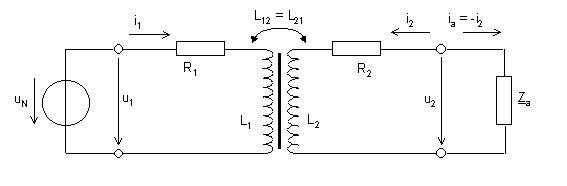
\includegraphics[width=0.7\linewidth]{./pics/el/trafo3}
						\caption{Ersatzschaltbild eines realen Transformators}
					\end{figure}\\
					Die Größen der Sekundärseite können auf die Primärseite mithilfe des Übertragungsfaktors $ \gamma $ umgerechnet werden.
					\[\gamma = \frac{N_{1}}{N_{2}} \quad \rightarrow \quad U'_{2}=U_{2}\gamma, \quad I'_{2}=\dfrac{I_{2}}{\gamma}, \quad L'_{\sigma2}=L_{\sigma2}\gamma^{2}, \quad \underline{Z}'=\underline{Z}\gamma^{2} \]
					Das heißt, ein sekundärseitiger Widerstand $ R $, wirkt primärseitig als $ R\gamma^{2} $.\\\\
					\begin{figure}[h]
						\centering
						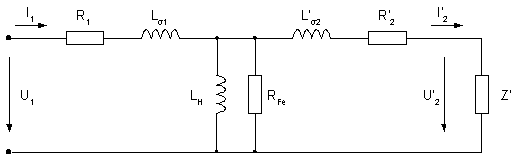
\includegraphics[width=0.7\linewidth]{./pics/el/trafo1.png}
						\caption{Ersatzschaltbild eines realen Transformators mit transformierten sekundärseitigen Größen}
					\end{figure}\\
					\tab[1cm] $R_{1}$\tab...\tab ohmscher Widerstand der Primärwicklung \\
					\tab[1cm] $R_{2}'$\tab...\tab transformierter ohmscher Widerstand der Sekundärwicklung \\
					\tab[1cm] $U_{1}$\tab...\tab primärseitige Spannungsquelle \\
					\tab[1cm] $U_{2}'$\tab...\tab transformierte Ausgangsspannung \\
					\tab[1cm] $Z'$ \tab...\tab transformierte Lastimpedanz \\
					\tab[1cm] $L_{\sigma 1}$\tab...\tab Streuinduktivität der Primärseite \\
					\tab[1cm] $L'_{\sigma 2}$\tab...\tab transformierte Streuinduktivität der Sekundärseite \\
					\tab[1cm] $L_{H}$\tab...\tab Hauptinduktivität, die den Magnetisierungsstrom führt \\
					\tab[1cm] $R_{fe}$\tab...\tab Eisenverluste des Kerns \\
					
				
		\subsection{Elektrische Aktuatoren}
			\leavevmode\\
			\textbf{\large Unterschiede zwischen Eisenlose und eisenbehaftete Motoren\\\\}
			Bei eisenlosen Motoren werden die Wicklungen mit Epoxid vergossen (Luftspaltwicklung). Diese Motoren sind für sehr gleichförmige Bewegungen geeignet. Bei ihnen wird keine magnetische Anziehungskraft erzeugt.
			Bei eisenbehafteten Motoren hingegen werden die Wicklungen in einem Eisenkäfig fixiert. Eisenbehaftete Motoren nutzen das Eisen, um den magnetischen Fluss zu bündeln und können so eine sehr hohe Kraftdichte erzeugen.\\\\			
			\textbf{Vorteile eisenlose Motoren:}
			\begin{itemize}
				\item Keine Eisenverluste (Eisenmagnet muss nicht umgepolt werden, die Hysteresekurve muss nicht durchlaufen werden, was Energie kostet)
				\item Kompakter und leichterer Forcer/Rotor
				\item Kleine Rotor Induktivität (weniger Elektromagnetische Störungen, schnelle Reaktionszeit des Stroms)
				\item Bei Sinuskommutierung erhält man ein gleichförmiges Moment bzw. eine konstant wirkende Kraft
			\end{itemize}
			\leavevmode \\
			\textbf{Vorteile eisenbehaftete Motoren:}
			\begin{itemize}
				\item sehr hohe Drehmomentdichte
				\item Maximierung der magnetischen Kraft
				\item höhere Spitzenkraft als eisenlose Motoren der selben Baugröße ($ \rightarrow $ kompaktere Ausführungen möglich)
			\end{itemize}
			
			\newpage	
			\subsubsection{Linearaktuatoren}				
				\begin{description}[leftmargin=2.5cm]
					\item[Allgemein]					
					Grundsätzlich arbeiten Linearmotoren wie rotatorische Motoren. Man kann sie sich so vorstellen, dass man einen beliebigen Motor aufschneidet und in die Ebene abwickelt.
					\leavevmode \\
					\begin{figure}[h!]
						\centering \rule{1.5cm}{0cm}
						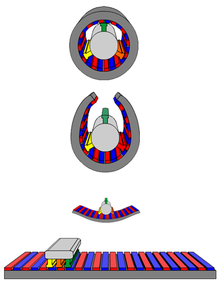
\includegraphics[width=0.2\linewidth]{./pics/el/rot2lin} 
					\end{figure} 
					Wobei die ursprünglich kreisförmig angeordneten elektrischen Erregerwicklungen (Stator) auf einer ebenen Strecke angeordnet sind. Der Läufer, der im Drehstrommotor rotiert, wird beim Linearmotor von dem längs bewegten Magnetfeld über die Fahrstrecke bewegt. Analog dazu funktionieren tubulare Linearmotoren ebenfalls wie ihre rotativen Verwandten, jedoch ist bei Linearmotoren der Untershied einer begrenzten Stator-Streke. Die Idee bei Linearmotoren ist, dass die durch den Motor erzeugte Kraft direkt auf eine zu bewegende Masse wirkt ohne Verluste in Getrieben, Spindeln, Riementrieben, usw. in kauf nehmen zu müssen.
					\begin{figure}[h!]
						\centering 
						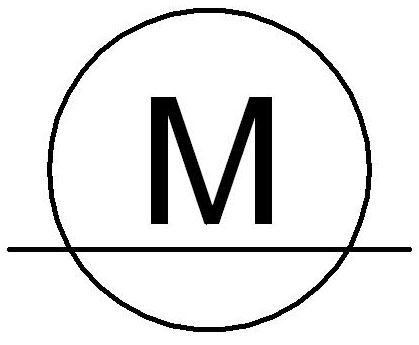
\includegraphics[width=0.05\linewidth]{./pics/el/symbolLinearmotor}
						\caption{Symbol für Linearmotoren}
					\end{figure} \leavevmode \\

					\item[Einteilung]
					\leavevmode \\
					\begin{figure}[h!]
						\centering
						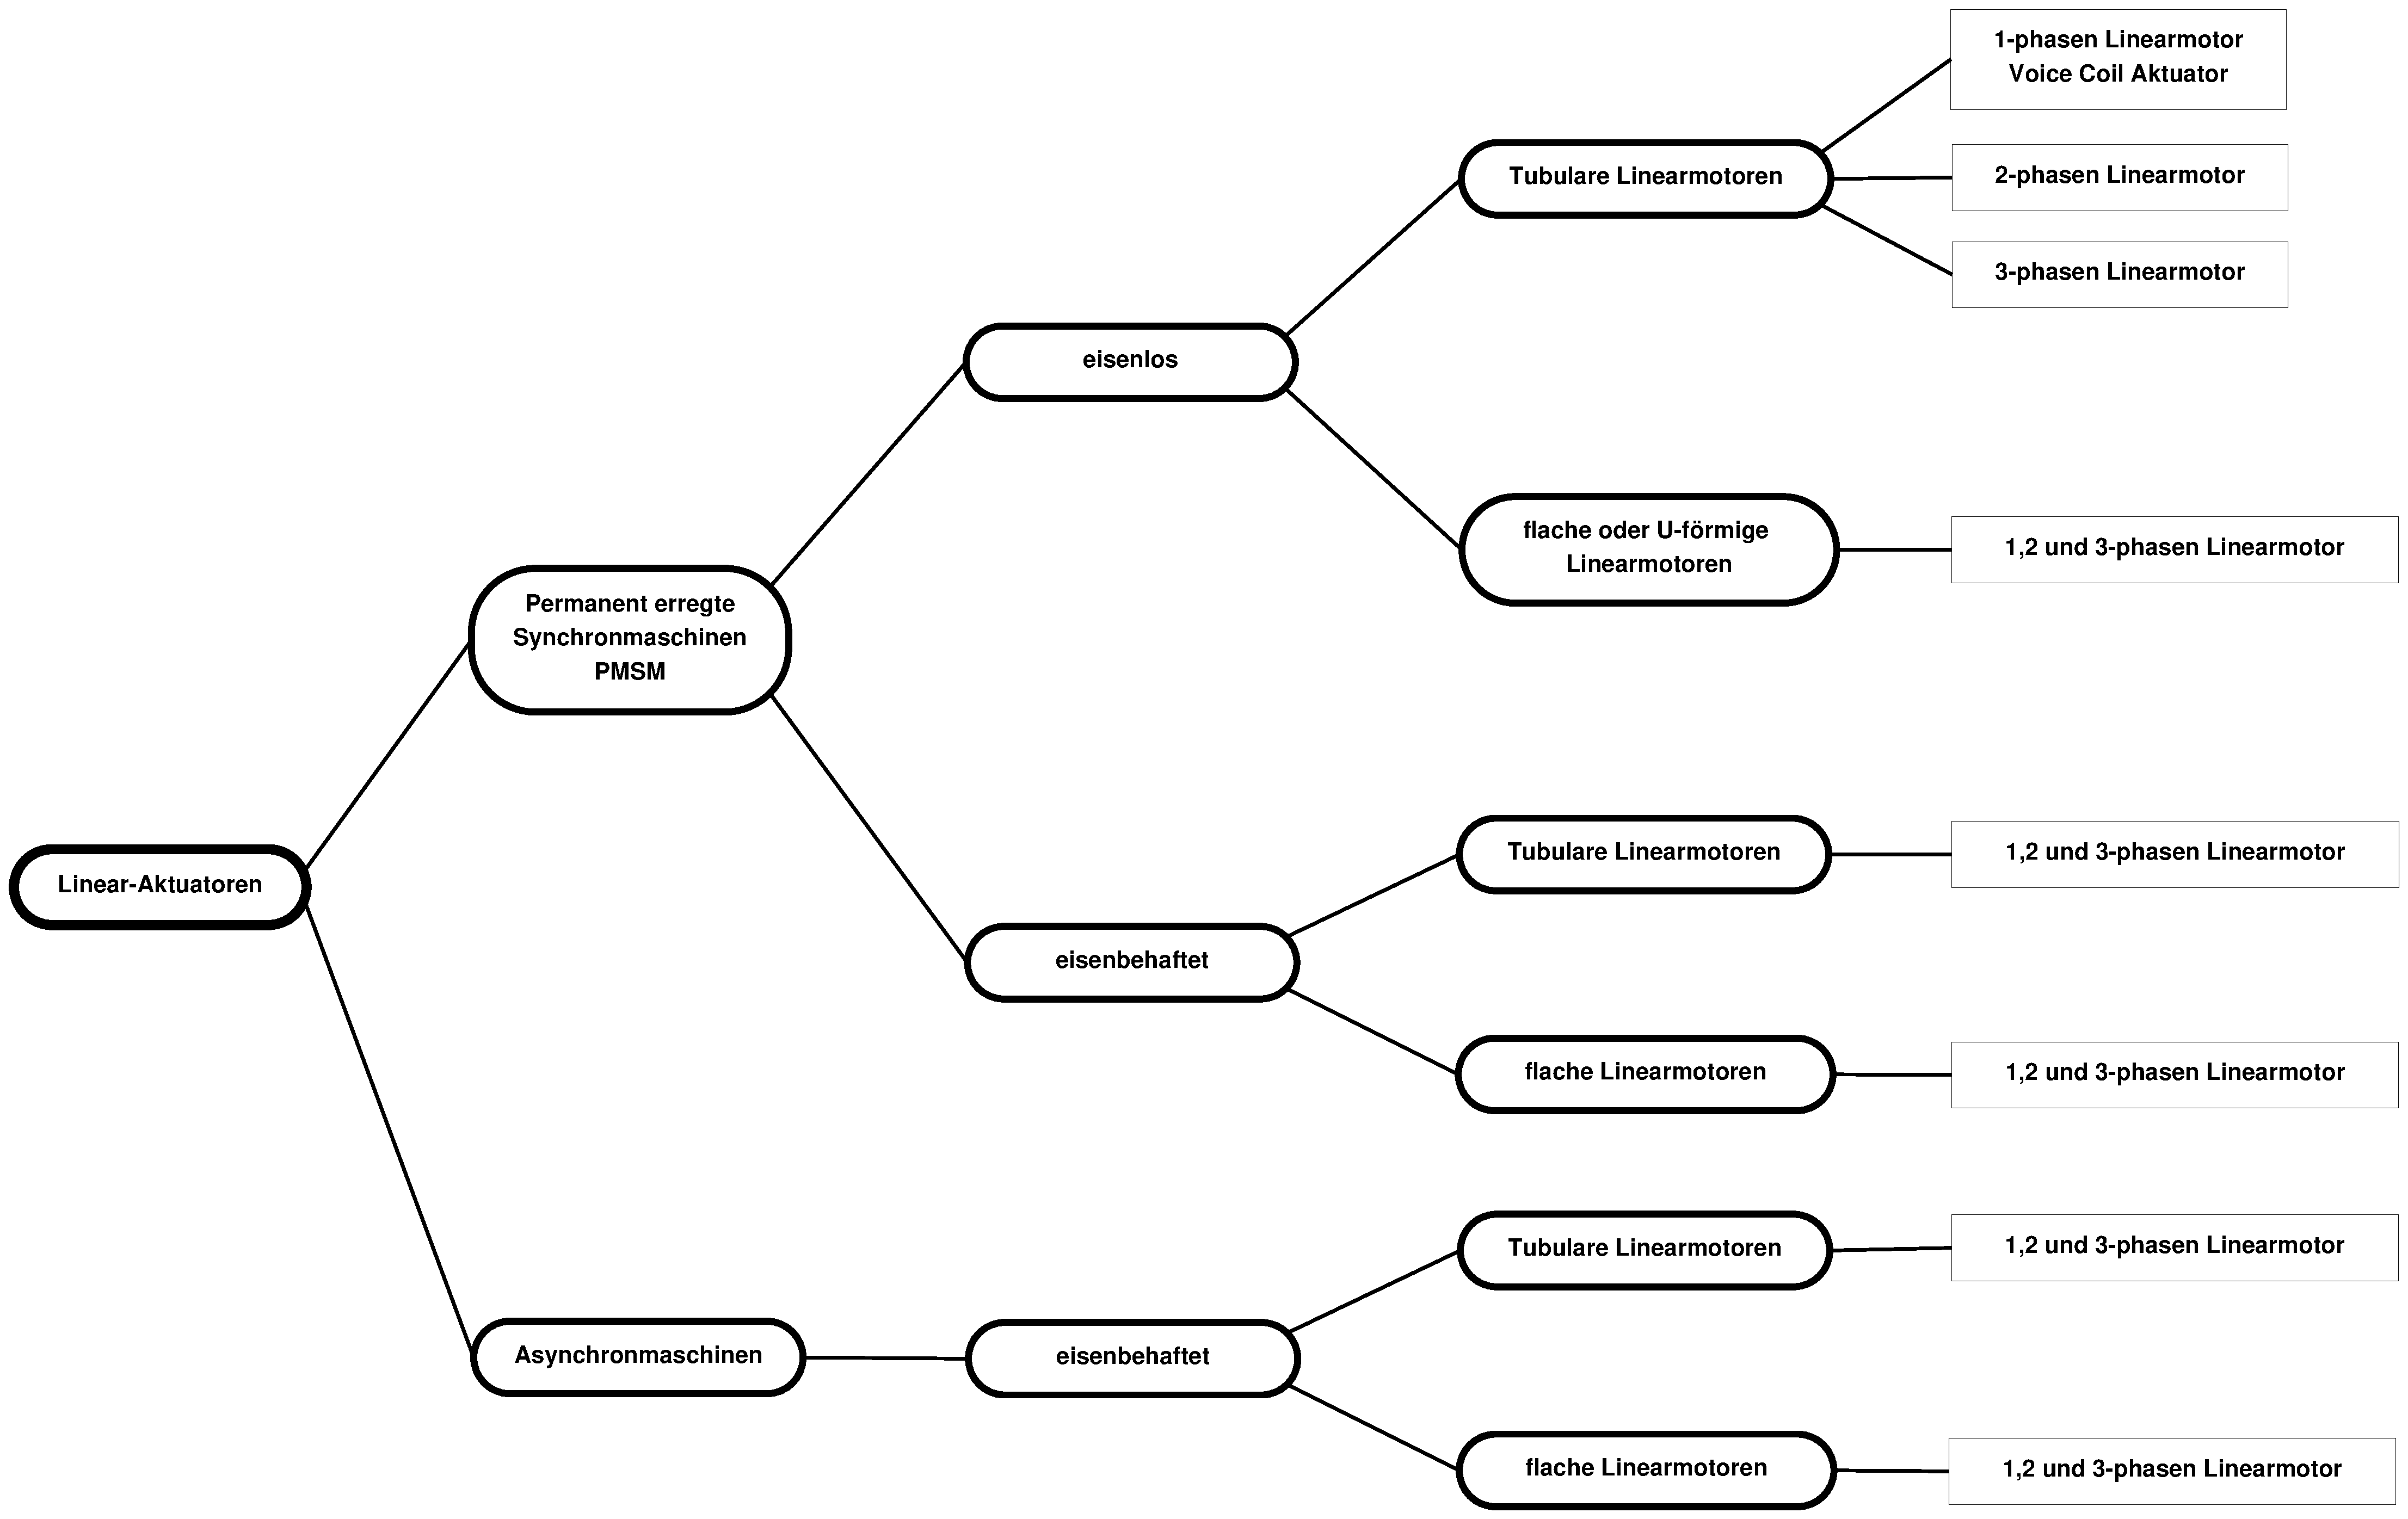
\includegraphics[width=0.9\linewidth]{./pics/el/LinearAktuatoren.eps}
					\end{figure}
				
					\item[Tubulare Linearmotoren] 
					Unter einem tubularen Linearmotor versteht man einen elektrischen Direktantrieb, bei dem die lineare Bewegung direkt aufgrund der elektromagnetischen Kraftwirkung erzeugt wird. Das heißt, die translatorische Bewegung wird nicht durch eine mechanische Umwandlung über eine Spindel, Riemen oder Kurvenscheibe erzeugt, sondern basiert direkt auf den Wechselwirkungen zwischen elektromagnetischen Kräften. Grundsätzlich können derartige Motoren sowohl nach dem Lorenzkraftprinzip wie auch nach dem Maxwellkraftprinzip (siehe Kap. \ref{reluktanzkraft}) aufgebaut werden und gehören zu der Gattung der Linearmotoren. Der Unterschied zu den flachen oder U-förmigen Linearmotoren besteht darin, dass die Erregerwicklung des Stators rohrförmig (tubular) und die Magnete des Läufers stabförmig sind. Konstruktiv gesehen entsteht so ein Antriebselement, das Ähnlichkeiten zu einem pneumatischen oder hydraulischen Zylinder aufweist. Im Bild ist ein permanenterregter Läufer abgebildet. Im asynchronen Fall besteht der Läufer statt aus Permanentmagneten, aus kurzgeschlossenen Kupferwindungen wie beim bekannten rotativen Asynchronmotor.
					\begin{figure}[!h]
						\centering \rule{1.5cm}{0cm}
						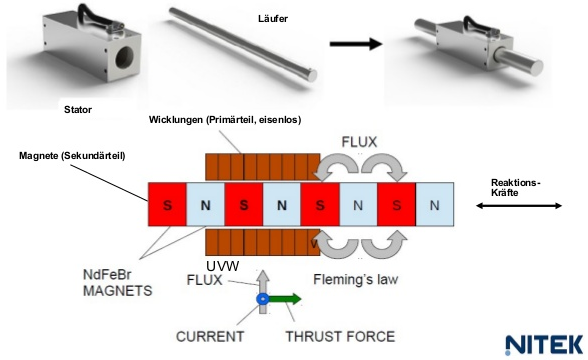
\includegraphics[width=0.55\linewidth]{./pics/el/tubular}
					\end{figure}
					
					\item[Flache, U-förmige Linearmotoren] 
					Bei flachen bzw. U-förmigen Linearmotoren befinden sich bei PMSM die Permanentmagneten am Stator des Motors. Beim asynchronen Linearmotor hält der Stator hingegen die Erregerwicklungen, die um weichmagnetisches Eisen gewickelt sind und somit Magnetfelder erzeugt.	Ein Linearmotor besteht aus nur zwei Komponenten: einem Wicklungspaket (Forcer bzw. Primärteil) und einem Träger (Magnetschiene bzw. Sekundärteil), auf dem die Permanentmagneten fixiert sind. Die Kupferwindungen des Wicklungspaketes sind entweder in Epoxidharz oder Eisen eingebettet. Die Kupferwindungen führen den gesamten Strom eines Linearmotors. 	
					\begin{figure}[h]
						\centering \rule{2.5cm}{0cm}
						\subfigure[U-förmiger Linearmotor]
						 {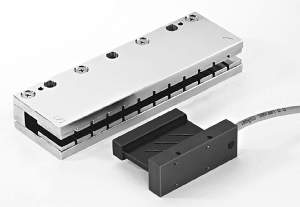
\includegraphics[width=0.4\textwidth]{./pics/el/LM}} \hspace{0.4cm}
						\subfigure[flacher Linearmotor] 
						 {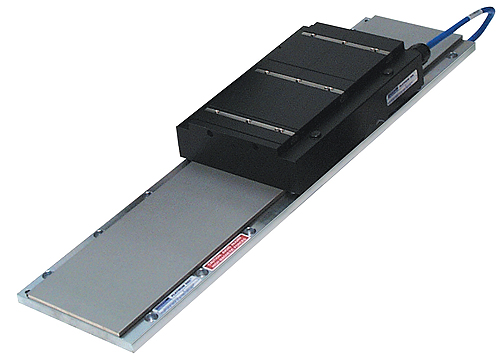
\includegraphics[width=0.4\textwidth]{./pics/el/flatLM}}
					\end{figure}					
					Das Magnetassembly besteht aus Seltenen-Erde-Magneten, die in abwechselnder Polarität auf einem Stahlträger montiert sind. Sie erzeugen ein magnetisches Feld senkrecht zum Träger. Wenn in den Kupferwindungen Strom fließt, ergibt sich nach dem Lorentz´schen Gesetz eine Kraft $ F = I \times B $, die zur Beschleunigung der Masse benutzt wird. Eine Linearmotorachse besteht wiederum aus einem Linearmotor mit Lagerung und einem integrierten Positions-Gebersystem (Encoder). Der Forcer wird üblicherweise an den bewegten Teilen der Maschine befestigt. Das Magnetassembly wird am statischen Teil der Maschine fixiert. 
					\begin{figure}[h]
						\centering \rule{2.5cm}{0cm}
						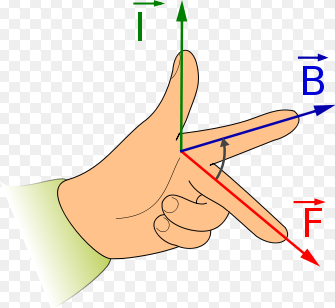
\includegraphics[width=0.2\linewidth]{./pics/el/I.png} \hspace{1cm}
						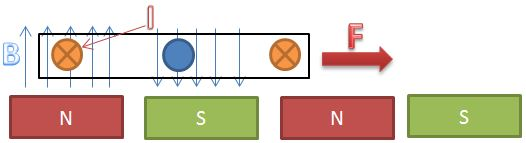
\includegraphics[width=0.5\linewidth]{./pics/el/LM2} 
						\caption{Linke-Hand-Regel für die Wirkrichtung der Lorentzkraft}
						\label{}
					\end{figure}
					
					\item[Asynhroner Linearmotor] 
					Beim linearen Asynchronmotor wird die bewegende Kraft durch ein wanderndes Magnetfeld das mit einem Leiter interagiert, erzeugt. In jedem Leiter, sei es eine Windung, Spule oder einfach nur eine leitende Metallplatte, die im Feld platziert wird, werden Ströme induziert. Durch Wechselwirkung des magnetischen Wanderfeldes und dem induzierten Strom resultiert jene Kraft, die für eine Linearbewegung verantwortlich ist. Asynchrone Linearmotoren werden für Anwendungen die große Kräfte benötigen verwendet. Zum Beispiel elektrisch Schiebetüren oder Magnetschwebebahnen.
					
					\item[PSM als Linearmotor] 
					Die permanenterregte Synchronmaschine (PSM) als Linearmotor benötigt im Forcer einen sinusförmigen Stromverlauf um ohne rucken bewegt werden zu können. Dies kann entweder durch Einspeisung von Wechselstrom erreicht werden oder durch Sinuskommutierung einer Gleichspannung. 
					
					\item[Sinuskommutierung]										
					Ein hoher Gleichlauf kann erreicht werden, indem die Phasenströme graduell angeglichen werden. Der Linearmotor ist geometrisch so aufgebaut, dass sich die Back-EMF in Form einer Sinusspannung ergibt. Daher ist die beste Lösung einen sinusförmigen Stromverlauf vor zu gegeben, der dann zu einer gleichmäßigen Bewegung führt. Das erzeugte Drehmoment/ die erzeugte Kraft ist dann konstant. Einen sinusförmigen Strom nachzubilden verlangt aber eine höhere Positionsauflösung als von den Hallsensoren erhalten werden kann. Der Strom in den 3 Phasen muss viel häufiger angepasst werden. Darum verwendet die Sinuskommutierung meist Encoder zur präzisen Lagebestimmung des Rotors. Sinuskommutierung ermöglicht einen gleichmäßigen Motorbetrieb und ergibt sogar eine bessere Performance.						
				\end{description}
				
				\paragraph{1-phasen Linearmotor/ Linear Voice Coil Motor/ Tauchspulenaktuator}
					Der Voice Coil Aktor ist ein zweipoliger nichtkommutierter Antriebsmechanismus mit limitiertem Weg. Er besteht aus zwei Komponenten: einem Dauermagneten am fixierten Teil und einer Spule, die auf einen im Luftspalt beweglichen nichtmagnetischen Spulenkörper gewickelt ist. Im eingebauten Zustand befindet sich die Spule im Luftspalt des Magnetfeldes. Richtung und Amplitude der Lorentzkraft werden dabei von der Stromstärke und -richtung bestimmt. Sie arbeiten nach dem Lorentz-Kraft-Prinzip und sind dadurch bidirektional aktiv ansteuerbar. Die konstante Kraftverteilung über dem Hub ermöglicht eine hohe Startkraft, die verbunden mit der geringen Masse der bewegten Spule höchste Dynamik erlaubt. Zudem lässt sich eine extrem geringe Hysterese erreichen. Durch diese Eigenschaften empfehlen sich Tauchspulenaktuatoren vor allem für dynamische und präzise Regelungsanwendungen.
					\begin{figure}[h]
						\centering
						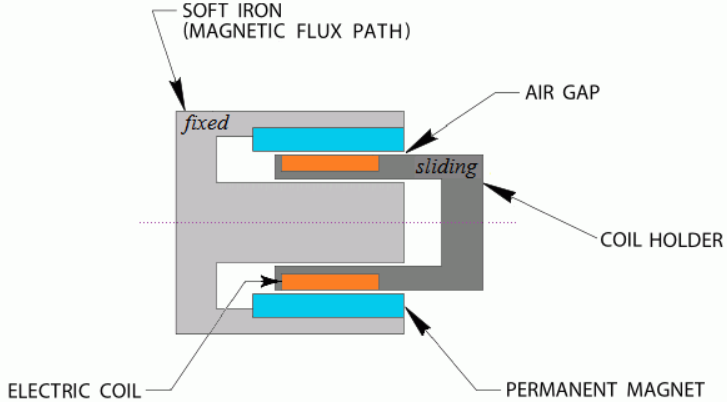
\includegraphics[width=0.6\linewidth]{./pics/el/vcm}
					\end{figure}
					\leavevmode \\
					
				\paragraph{2- und 3-phasen Linearmotor} 
					\begin{description}[leftmargin=2.5cm]
						\item[Bsp. 2-phasen Linearmotor]
						Das Funktionsprinzip ist das selbe wie im Kapitel Linearmotoren erklärt wird. In der Abbildung funktioniert der eisenbehaftete LM nach dem Reluktanzkraft-Prinzip (Kap. \ref{reluktanzkraft}).	\\
						\begin{figure}[h]
							\centering
							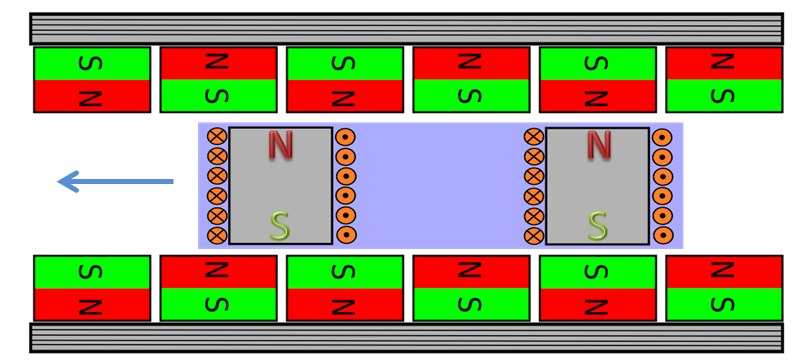
\includegraphics[width=0.6\linewidth]{./pics/el/2phase}
							\caption{2-phasiger, eisenbehafteter, U-förmiger Linearmotor}
						\end{figure} \\
						Die Magnetfelder des Läufers und die des Stators werden immer kombiniert geschaltet (mit Strom versorgt), dass der Läufer vom nächsten Permanentmagnetpol in Bewegungsrichtung ein Wegstück „nach vorne“ gezogen wird (und vom Magnetfeld hinter sich abgestoßen wird). Hat er die Position erreicht, zu der er gezogen wurde, so wird umgepolt, und der Läufer wird von dieser Position nun weggedrückt und zur nächsten Magnetspule/Permanentmagnet hingezogen. Dadurch, dass der Läufer zwei etwas versetzte Magnetfeld-Erzeuger besitzt, befindet sich immer mindestens einer davon gerade „auf halbem Weg“, was eine Festlegung der Laufrichtung (vorwärts oder rückwärts) ermöglicht. Dieser Motor ist die lineare Variante einer permanenterregten Synchronmaschine.
						
						\item[Bsp. 3-phasen Linearmotor]
						Die eisenlosen 3-phasigen elektronisch kommutierten AC synchron
						Linearmotoren sind für die anspruchsvollen Anforderungen
						mit hohen Beschleunigungen sehr gut geeignet. Vorteil der 3-phasigen Linearmotoren ist, dass ein gleichmäßigerer Lauf möglich ist bzw. eine konstante Kraft geliefert werden kann.
						\begin{figure}[h]
							\centering
							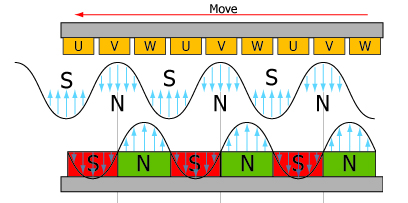
\includegraphics[width=0.7\linewidth]{./pics/el/3phaseLin}
							\caption{eisenloser, permanenterregter, 3-phasen synchron Linearmotor}
						\end{figure}
					\end{description}
					
			\subsubsection{Rotationsaktuatoren}
				\paragraph{Gleichstrommotoren} 
					\subparagraph{Brushless DC-Motor}
						\begin{description}[leftmargin=3cm]
							\item[Aufbau] 
							Der \textit{brushless DC-Motor} basiert entgegen der Namensgebung nicht auf dem Funktionsprinzip der Gleichstrommaschine, sondern ist aufgebaut wie eine Drehstrom-Synchronmaschine mit Erregung durch Permanentmagnete. Die (oft dreisträngige) Drehstromwicklung wird elektronisch kommutiert (z.b. Block- oder Sinuskommutierung). Dadurch entsteht ein sich drehendes magnetisches Feld, welches den permanenterregten Rotor mitzieht.
							\begin{figure}[h]
								\centering \rule{3cm}{0cm}
								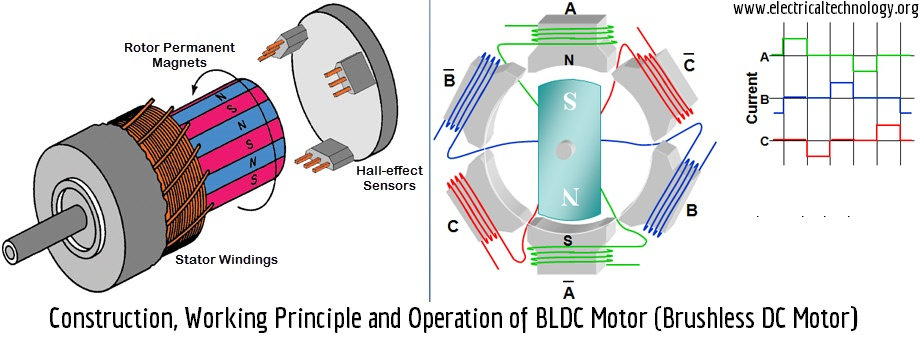
\includegraphics[width=0.82\linewidth]{./pics/el/brushless}
							\end{figure}
							\item[Kommutierungsarten]
							Bei einer Blockkommutierung wird der Strom in den jeweiligen Wicklungen zwischen 3 Zuständen geschaltet. Das sich dabei ergebende Drehmoment weist eine Welligkeit auf. Bei einer Sinuskommutierung ergibt sich hingegen ein konstantes Drehmoment. Die Kommutierung kann entweder mit oder ohne Sensoren erfolgen.
							\begin{figure}[h]
								\centering \rule{1cm}{0cm}
								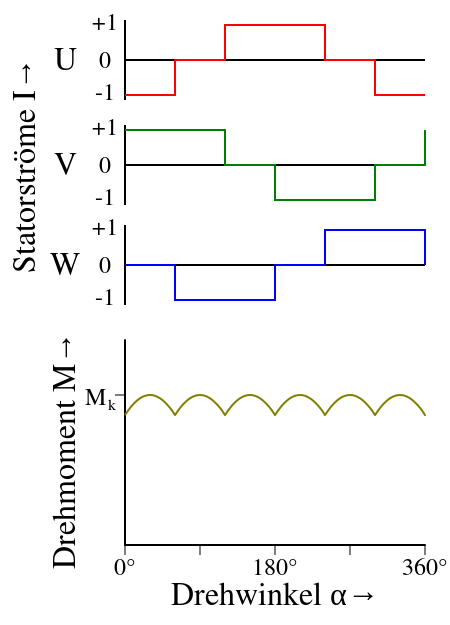
\includegraphics[width=0.3\linewidth]{./pics/el/blockkomm}
							\end{figure} 
							
							\item[Sensorgesteuerte Kommutierung]
							Bei ersterem werden entweder Hallsensoren oder optische Sensoren verwendet.	Entsprechend dieser Stellungsinformation werden über geeignete Leistungstreiber von der Steuerelektronik die Wicklungen angesteuert, die im Rotor ein Drehmoment erzeugen. Der Vorteil ist, dass die sensorgesteuerte Kommutierung auch bei sehr geringen Drehzahlen bzw. im Stand funktioniert. Gewöhnlich werden bei dieser Kommutierung nicht alle Phasen zugleich bestromt. Bei den Dreiphasenmotoren ist üblicherweise zu jedem Zeitpunkt jeweils eine Phase stromlos.
							
							\item[Sensorlose Kommutierung]
							Bei der sensorlosen Kommutierung erfolgt die Erfassung der Rotorposition über die in den Spulen des Stators induzierte Spannung, welche von der elektronischen Steuerschaltung ausgewertet wird. Allerdings ist zur Auswertung der Induktionsspannung eine gewisse Mindestdrehzahl erforderlich. Sensorlose EC-Motoren müssen daher wie Synchronmotoren bzw. Schrittmotoren bis zum Erreichen der Mindestdrehzahl blind geschaltet werden.
							Mittlerweile gibt es allerdings Verfahren, mit denen ein EC-Motor auch unterhalb dieser Mindestdrehzahl nicht blind gesteuert wird. Dazu werden bei Stillstand kurze Stromimpulse gesendet, die den Motor zwar nicht bewegen, aber durch das magnetische Feld des Rotors beeinflusst werden. Das Magnetfeld mindert oder verstärkt den Stromfluss und verändert so die Zeit, die ein Stromimpuls benötigt, um eine Schwelle zu überschreiten. Diese Zeiten werden gemessen, und man kann damit die Rotorposition schon bei Stillstand bestimmen.
							
							\item[Geeignetste Kommutierung]
							Man erhält für EC-Motoren (electronically commutated) das beste Ergebnis (konst. Kraft), wenn man sie mit ihrer BEMF-Spannung (back electromotive force) ansteuert. Diese Spannung kann an bzw. zwischen den Phasen gemessen werden, wenn man den Motor von Hand bewegt.
							
							\item[Unterschied zur PMSM]
							Die BEMF ergibt bei PMSM einen sinusoidalen Spannungsverlauf. Bei BLDC hingegen einen trapezförmigen Spannungsverlauf der Gegeginduktionsspannung. Die Verläufe folgern aus den unterschiedlichen Statorwicklungen. Bei BLDC sind die Wicklungen konzentriert und bei PMSM hingegen viel gleichmäßiger auf den Umfang verteilt, was zu einer sinusoidalen Spannung führt. Dadurch Unterscheidt sich auch die Ansteuerung der beiden Motoren, da man die höchste Performance erreicht indem man den Motor mit der selbigen Spannung als seine BEMF ansteuert.
							\begin{figure}[h]
								\centering 
								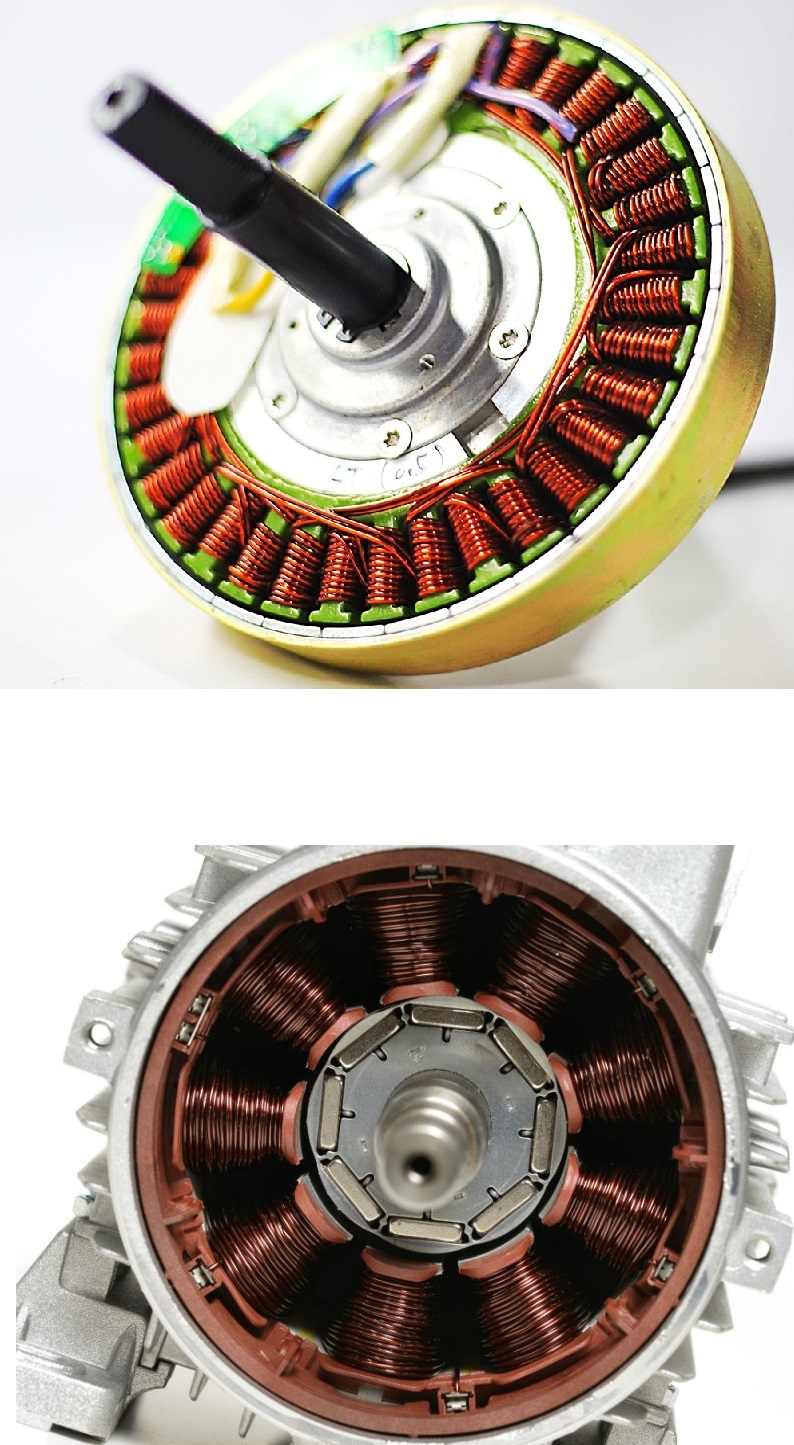
\includegraphics[width=0.27\linewidth]{./pics/el/bldcpmsm}
								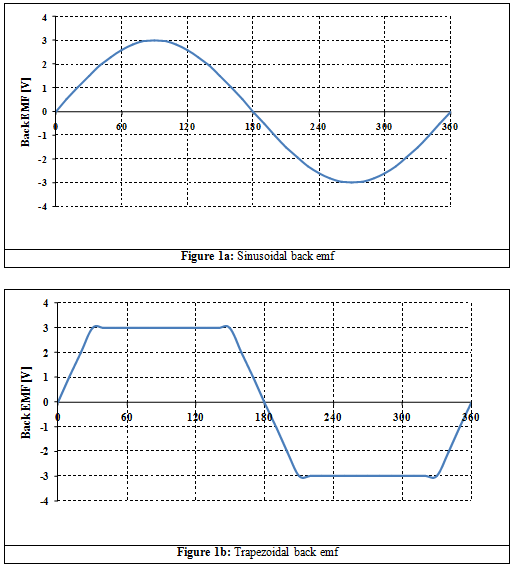
\includegraphics[width=0.45\linewidth]{./pics/el/sinus}
								\caption{PMSM- sinusoidale BEMF}
							\end{figure}
						\end{description}
	
					\subparagraph{Steppermotor}
						\begin{description}[leftmargin=3cm]
							\item[Allgemein]
							Ein Schrittmotor ist ein Synchronmotor, bei dem der Rotor  durch ein gesteuertes, schrittweise rotierendes, elektromagnetisches Feld der Statorspulen um einen minimalen Winkel (Schritt) oder sein Vielfaches gedreht werden kann. Schrittmotoren existieren auch in Form von Linearmotoren. Schrittmotoren folgen im Prinzip exakt dem außen angelegten Feld und können ohne Sensoren zur Positionsrückmeldung (Encoder, Drehgeber oder ähnliches) genau betrieben werden. Sie sind haben ein ähnliches Verhalten wie Synchronmotoren, weisen aber in der Regel eine deutlich höhere Polpaarzahl auf. Daher können sie einfacher betrieben werden als beispielsweise Servomotoren, da diese auf die gewünschte Position eingeregelt werden müssen. Für einen besonders homogenen Verlauf werden Schrittmotoren mit einem gleichförmigen Drehfeld angesteuert.
							\begin{figure}[h]
								\centering \rule{2.5cm}{0cm}
								\subfigure[Schema mit 4 Schritten pro Umdrehung und unipolarer Beschaltung]
								{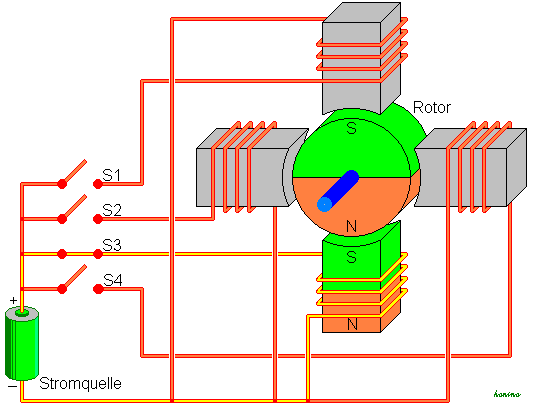
\includegraphics[width=0.45\textwidth]{./pics/el/stepper}} \hspace{0.4cm}
								\subfigure[Reluktanzschrittmotor] 
								{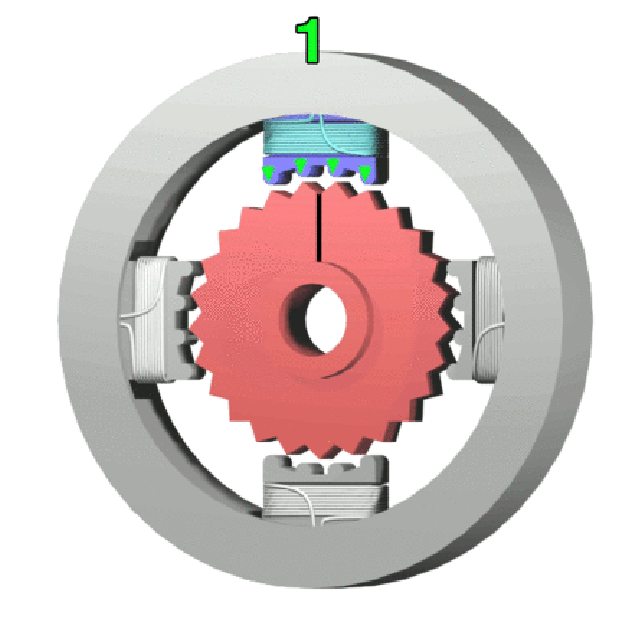
\includegraphics[width=0.35\textwidth]{./pics/el/StepperMotor.png}}
							\end{figure}	
							
							\item[Schrittverlust] 
							Wird ein Schrittmotor durch ein externes Lastmoment oder durch die anzutreibende Masse beim starken Beschleunigen beziehungsweise Verzögern überlastet (d. h. Lastmoment > Motormoment), kann der Rotor dem Drehfeld nicht mehr folgen. Es werden Schritte übersprungen, und die Information über die aktuelle Position des Rotors geht verloren. Bei diesem sogenannten Schrittverlust springt der Motor in die vorherige oder nächste Position gleicher Phase zurück. Durch die mechanische Bewegungsenergie (Trägheit) kommt es bei rasch bewegten Magnetfeldern meist zu einer Serie von verlorenen Schritten. Auftretende Schrittverluste summieren sich und führen dann zu einer ungenauen Positionierung.
							
							\item[Bauarten]
							\begin{itemize}
								\item Reluktanzschrittmotor
								\item Permanentmagnetschrittmotor
								\item Hybridschrittmotor (Reluktanz- und Permantmagnetschrittmotor)
								\item Lavet-Schrittmotor
							\end{itemize}
						
							\item[Reluktanzschrittmotor]
							Beim Reluktanzschrittmotor besteht der Rotor aus einem gezahnten Weicheisenkern. Bei diesem Material verschwindet nach dem Ausschalten des Statorstromes das Magnetfeld. Bei eingeschaltetem Strom fließt der magnetische Fluss durch den Weicheisenkern des Rotors. Die Drehbewegung des Rotors kommt zustande, weil vom gezahnten Stator der nächstliegende Zahn des Rotors angezogen wird, da sich so der magnetische Widerstand verringert. Da der Reluktanzschrittmotor keine Permanentmagnete enthält, hat er daher im Gegensatz zum Permanentmagnetschrittmotor bei ausgeschaltetem Strom auch kein Rastmoment.
							
							\item[Permanentmagnetschrittmotor]
							Beim Permanentmagnetschrittmotor besteht der Stator aus Weicheisen und der Rotor aus Dauermagneten, die abwechselnd einen Nord- und einen Südpol aufweisen. Mit dem Stator-Magnetfeld richtet man den dauermagnetischen Rotor so aus, dass eine Drehbewegung entsteht. Beim Permanentmagnetschrittmotor ist die Anzahl der Pole (und damit die Auflösung) begrenzt.
							
							\item[Hybridschrittmotor]
							Der Hybridschrittmotor vereint die positiven Eigenschaften beider Bauformen durch feine Schrittteilung und gutes Drehmoment. Sein Rotor besteht aus einem axialen Permanentmagneten, an dessen Enden (Polen) gezahnte Weicheisenkränze befestigt sind. Beide sind um eine halbe Zahnbreite gegeneinander versetzt, so das sich Nord- und Südpole abwechseln. Vorteil ist das erheblich kleinere äußere Magnetfeld. Nahezu alle heute erhältlichen Schrittmotoren sind Hybridmotoren, da er hohe mechanische Leistungen bei kleinen Schrittwinkeln und kleiner Bauform vereint. Die gebräuchlichsten Schrittauflösungen liegen zwischen 50 und 2000 Schritte pro Motorumdrehung ohne elektronische Zusatzmaßnahmen. Bezüglich der Phasenzahl sind 2-Phasenmotore am gängigsten.
							\begin{figure}[h]
								\centering \rule{1.5cm}{0cm}
								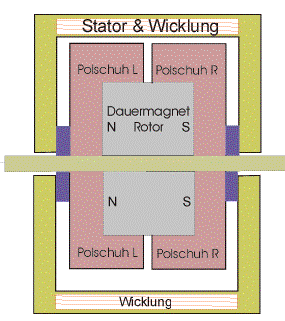
\includegraphics[width=0.4\linewidth]{./pics/el/hybrid}
							\end{figure}
						
							\item[Ansteuerung \& Anschluss]
							Weiterhin kann man zwei Gruppen von Motoren bzw. Ansteuertechniken unterscheiden: Unipolare und bipolare Motoren. Unipolare Motoren verfügen über zwei Spulen mit Mittelabgriff. Sie haben fünf oder sechs Anschlüsse. Mit einem Multimeter läßt sich schnell feststellen, welche Anschlüsse die Mittelabgriffe und welche die Spulenenden sind. Die Ansteuerung erfolgt durch wechselweises Einschalten von jeweils einem Spulenende, so daß immer nur die halbe Spule bestromt ist.
							Ein 2-phasiger, bipolarer Motor hat zwei Spulen, manchmal auch zwei Spulenpaare, die durch Umpolen angesteuert werden. Sind zwei Spulenpaare vorhanden (also acht Anschlüsse am Motor), können die Spulenpaare wahlweise parallel oder in Reihe geschaltet werden, woraus sich unterschiedliche (dynamische) Eigenschaften ergeben. Eine Parallelschaltung führt im allgemeinen zu mehr Drehmoment im oberen Drehzahlbereich, stellt aber auch höhere Anforderungen an den Stromregler. Bipolare Motoren mit 8 Anschlüssen können prinzipiell auch unipolar angesteuert werden, wobei man allerdings einen Teil der Motorperformance verschenkt.
							\begin{figure}[h]
								\centering \rule{1.5cm}{0cm}
								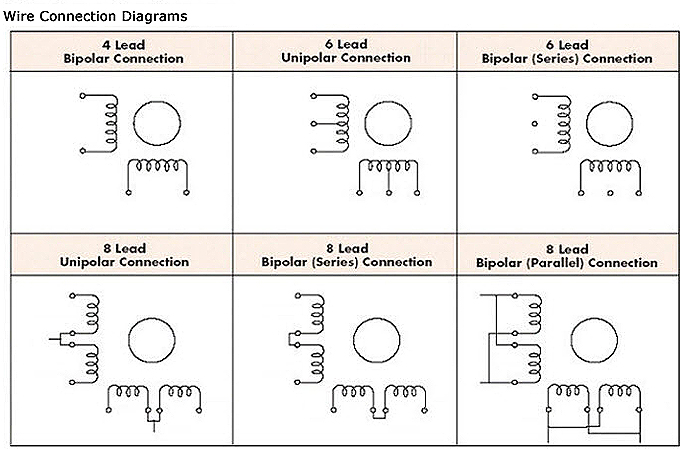
\includegraphics[width=0.7\linewidth]{./pics/el/unibipolar}
								\caption{Anschlussvarianten eines 2-phasigen Steppermotors}
							\end{figure} 
							Bei der Beschaltung der Spulen ergeben sich drei weitere Betriebsarten: Vollschritt- Wavedrive- und Halbschrittbetrieb.
							\begin{enumerate}
								\item Normal-Betrieb: Es werden immer beide Spulen gleichzeitig bestromt. Es ergeben sich vier unterschiedliche Schrittpositionen (siehe Schaubild) pro Umlauf.
								\item Wavedrive-Betrieb: Hier wird immer nur eine Spule bestromt. Die Leistungsaufnahme und damit auch das Drehmoment sind im Vergleich zu 1) geringer. Die resultierenden vier Schrittpositionen liegen zwischen denen aus 1).
								\item Halbschritt-Betrieb: Kombination aus 1) und 2). Es wird wechselweise eine, bzw. zwei Spulen bestromt. Es ergeben sich 8 Schrittpositionen. Daher kommt die Bezeichnung Halbschritt, da der physikalische Schrittwinkel des Motors halbiert wird.
							\end{enumerate}		
							\begin{figure}[h]
								\hspace{3.2cm}
								\begin{minipage}{0.75\textwidth}		
								\centering 
								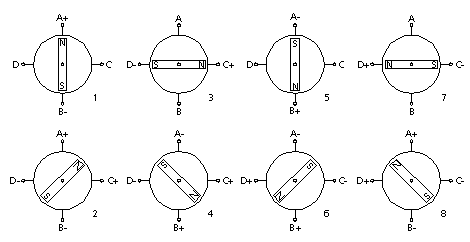
\includegraphics[width=1\linewidth]{./pics/el/vollschritt}
								\caption{Oberen vier Zustände: Wavedrive-Betrieb, unteren vier Zustände: Vollschrittbetrieb,		Halbschrittbetrieb: alle 8 Zustände}
								\end{minipage}
							\end{figure} 							
						
							\item[Vor- \& Nachteile gegenüber BLDC]
							\hspace{0.5cm}
							\begin{minipage}[t]{0.38\textwidth}
								\textbf{Steppermotor}
								\begin{itemize}
									\item[+] Günstiger als BLDC (Preis-Leistung)
									\item[+] Einfache Winkel-(Weg-)messung durch Schrittzählung ohne Encoder möglich
									\item[-] Moment nimmt ab einer bestimmten Drehzahl ab	
									\item[-] nur niedrige Drehzahlen möglich
																	
								\end{itemize}
							\end{minipage}
							\hspace{0.5cm}
							\begin{minipage}[t]{0.35\textwidth}
								\textbf{Brushless DC-Motor}
								\begin{itemize}
									\item[+] Hohe Drehzahlen
									\item[+] Sehr gute Laufruhe
									\item[+] günstiger Momentenverlauf über den gesamten zulässigen Drehzahlbereich
									\item[-] Kostet mehr als Stepper
									\item[-] Encoder nötig für Weg-, Drehzahlmessung
								\end{itemize}
							\end{minipage}	
						
							\item[Anwendungszwecke]
							Typische Anwendungsgebiete sind Drucker, vor allem Matrixdrucker, oder der Antrieb des Schreib-/Lesekopfes in einem Diskettenlaufwerk. Aufgrund ihrer hohen Genauigkeit werden sie auch in computergesteuerten Werkzeugmaschinen zur Positionierung der Werkzeuge verwendet. Durch die ständig sinkenden Kosten für die Ansteuerelektronik werden sie auch zunehmend im Konsumgüterbereich verwendet. So sind in Kraftfahrzeugen der mittleren und gehobenen Kategorie heute bis über 50 Schrittmotoren im Einsatz, die Betätigung der vielen Klappen einer automatischen Heizungs- und Klimaanlage ist dafür ein Beispiel. Schrittmotoren können bis ungefähr 1 kW wirtschaftlich eingesetzt werden.
																		
						\end{description}
						
					\subparagraph{Servomotor}
						Als Servomotor werden Elektromotoren beliebiger Bauart (AC, DC) bezeichnet, die die Kontrolle der Winkelposition, Drehzahl und Winkelbeschleunigung ihrer Motorwelle erlauben. Bürstenlose Servomotoren sind entweder Brushless DC-Motoren, Drehstrom-Asynchronmotoren oder Drehstrom-Synchronmotoren. Sie bestehen aus einem Elektromotor, der zusätzlich mit einem Sensor (Encoder) zur Positionsbestimmung ausgestattet ist. Die vom Sensor ermittelte Winkelposition/ -geschwindigkeit der Motorwelle wird kontinuierlich an eine meist außerhalb des eigentlichen Motors angebrachte Regelelektronik übermittelt, den so genannten Servoregler, der die Bewegung des Motors entsprechend einem oder mehreren einstellbaren Sollwerten, wie etwa Soll-Winkelposition oder Solldrehzahl, regelt.
						\begin{figure}[h]
							\centering
							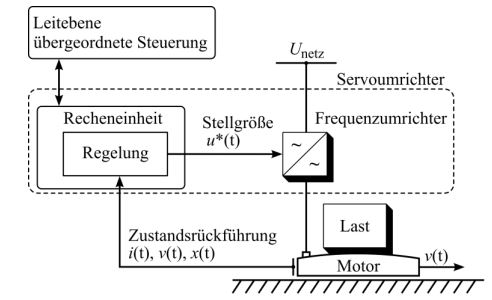
\includegraphics[width=0.5\linewidth]{./pics/el/servo}
							\caption{Die Kombination Servomotor und Servoregler wird als Servoantrieb bezeichnet}
	
						\end{figure}
						
					\subparagraph{Torque-Motor} 
						Torque-Motoren können als Außenläufer (Stator innen, Rotor außen) oder normale Innenläufer ausgeführt sein. Durch den verhältnismäßig großen Durchmesser, die hochpoligen Wicklungen können diese Motoren große Drehmomente bei geringen Drehzahlen erzeugen. Meist werden BLDC-Motoren als Torquemotoren gebaut, teilweise aber auch Reluktanzmotoren.
						\begin{itemize}
							\item[+] Große Beschleunigungen möglich $ \rightarrow $ hohe Dynamik des Systems
							\item[+] Antriebssteif $ \rightarrow $ kein Verdrehspiel $ \rightarrow $ geringere Störgrößen $ \rightarrow $ gute Regeleigenschaften
							\item[+] Kaum Verschleiß
							\item[-] Starke Wärmeentwicklung (muss oft Wassergekühlt werden)
							\item[-] Teuer
						\end{itemize}
						\begin{figure}[h]
							\centering
							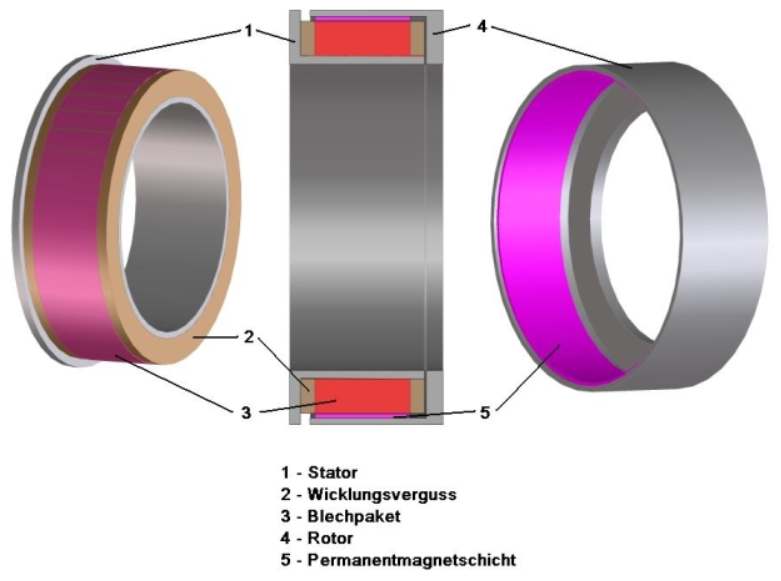
\includegraphics[width=0.5\linewidth]{./pics/el/TM}
						\end{figure}
						
				\paragraph{Drehstrommotoren} 
					\subparagraph{\textcolor{red}{Synchronmotor}}						
						Mn und Pn Kurven, vergleich mit asynchron!!!
					\subparagraph{\textcolor{red}{Asynchronmotor}}
				\paragraph{\textcolor{red}{Wechselstrommotoren}} 
					\subparagraph{\textcolor{red}{Reluktanzmotor}}
					\subparagraph{...}